\documentclass[english, LaM, oneside]{sapthesis}%remove "english" for a thesis written in Italian
%Bachelor's (laurea triennale) thesis : Lau 
%Master's (laurea specialistica) thesis: LaM 
%PhD's thesis: PhD 
%\usepackage[italian]{babel} %use this package for a thesis written in Italian
\usepackage[utf8]{inputenx}
\usepackage{indentfirst}
\usepackage{microtype}


\usepackage{fixltx2e}
\usepackage{stackengine}


% \usepackage{natbib}
% \bibliographystyle{plainnat} % You can choose other styles like "abbrvnat" or "unsrtnat"
% \usepackage{algpseudocode}
\usepackage{algorithm}
\usepackage{algorithmic}
\usepackage{amssymb}
\usepackage{adjustbox}

\usepackage{algpseudocode} 
\usepackage{booktabs}
\usepackage{cite}
\usepackage{subfig}
\usepackage{graphicx} %package to manage images
%\usepackage{chemformula}
%\usepackage{setspace}
%\usepackage{yfonts,color}
%\usepackage{siunitx}
%\usepackage{comment}
%\usepackage{multirow}
%\usepackage{varioref}
%\usepackage[bottom]{footmisc}
%\usepackage{wrapfig}
%\usepackage{float}
%\usepackage{type1cm}
\usepackage{lettrine}
\linespread{0.9}
%\usepackage{chngcntr}
\usepackage[nottoc, notlof, notlot]{tocbibind}
%\onehalfspacing
%\counterwithout{footnote}{chapter}


\usepackage{hyperref}
\hypersetup{
			hyperfootnotes=true,			
			bookmarks=true,			
			colorlinks=true,
			linkcolor=red,
                        linktoc=page,
			anchorcolor=black,
			citecolor=red,
			urlcolor=blue,
			pdftitle={A sample Bachelor's thesis for Sapienza Università di Roma},
			pdfauthor={FirstName LastName},
			pdfkeywords={thesis, sapienza, roma, university}
 }
% \courseorganizer{Facolt\`a di Ingegneria dell'informazione, informatica e statistics
% INGEGNERIA DELL'INFORMAZIONE, ELETTRONICA E TELECOMUNICAZIONI}
\title{A Deep Learning Architecture for Enhanced Depth Estimation on an unrectified Stereo 360$^{\circ}$ dataset}
\author{Danial Zendehdel}
\IDnumber{1903607}
\course[]{Ingegneria dell'informazione, elettronica e telecomunicazioni}
\courseorganizer{Facolt\`a di Ingegneria dell'informazione, informatica e statistics}
\submitdate{2022/2023}
\copyyear{2023}
\advisor{Prof. Antonello Rizzi}
\advisor{Prof. Alexandre Masoud Alahi}
\coadvisor{Dr. Enrico De Santis}
\authoremail{Zendehdel.d@gmail.com}
\examdate{29 May 2023}
% \examiner{Prof. ...} \examiner{Prof. ...} \examiner{Prof. ...}  \examiner{Prof. ...}  \examiner{Prof. ...} \examiner{Prof. ...}  \examiner{Prof. ...} 

%we refer to http://ctan.mirrorcatalogs.com/macros/latex/contrib/sapthesis/sapthesis-doc.pdf for an exhaustive description of the sapthesis documentclass.


\begin{document}

\frontmatter
\maketitle

\begin{abstract}

Stereo depth estimation is a critical problem in computer vision, with applications in robotics, self-driving vehicles, unmanned aerial vehicles, virtual and augmented reality, and 3D model reconstruction. While deep learning has led to significant improvements in depth estimation, existing datasets are predominantly synthetic and do not fully represent the complexity of real-world scenes or 360$^\circ$ images. This thesis presents a novel dataset for depth estimation from stereo 360$^\circ$ images and explores the challenges and opportunities it offers.

The dataset has several unique characteristics: it includes real-world images, features a vertical camera and LiDAR setup, contains unrectified image pairs, and provides depth images as ground-truth instead of disparity maps. These properties make the dataset more challenging and better suited for real-world applications.

We evaluate the performance of popular depth estimation architectures, such as PSMNet and 360SD-Net, on our dataset and identify their strengths and weaknesses in handling stereo 360$^\circ$ images. To further improve performance, we modify and add code to these architectures, demonstrating that our dataset presents a new challenge for deep learning tasks in stereo-depth estimation. By achieving satisfactory results at the primary level, we provide a foundation for future research in this area.

The thesis is organized into six chapters: Introduction, State of the Art, Proposed Dataset, Deep Learning Architectures, Experiments and Results, and Conclusion. The work presented in this thesis contributes to advancing the field of stereo depth estimation and paves the way for further exploration of the challenges and opportunities associated with real-world, stereo 360$^\circ$ images.


\end{abstract}

\newpage

\section*{Acknowledgements}

First and foremost, I would like to express my deepest gratitude to my main supervisor, Prof. Antonello Rizzi, for his invaluable guidance, support, and mentorship throughout the course of my thesis. His expertise and insights have been crucial to the development and completion of this work. I am grateful for the countless hours he dedicated to discussing ideas, providing feedback, and encouraging me to strive for excellence in my research.

I would also like to thank my second supervisor, Prof. Alex Masoud Alahi, for his valuable contributions and suggestions, which have significantly enriched the quality of my research. His expertise in the field of computer vision and deep learning has been instrumental in shaping the direction of my thesis.

I am grateful to the EPFL University and the VITA-lab for providing an excellent research environment, state-of-the-art facilities, and access to cutting-edge resources. The stimulating and collaborative atmosphere at the VITA-lab has been an invaluable source of motivation and inspiration for my work.

I would like to extend my appreciation to all the faculty members, lab mates, and fellow students who have contributed to my academic and personal growth during my time at EPFL. Their support, friendship, and camaraderie have made this journey truly memorable.

Finally, I would like to express my profound gratitude to my family and friends for their unwavering support, love, and encouragement throughout my academic pursuits. They have been my rock and my constant source of strength, and I dedicate this thesis to them.


\tableofcontents

\listoffigures
\listoftables
\mainmatter
\chapter{Introduction}

% \lettrine[lines=2, findent=3pt, nindent=0pt]{D}{}epth estimation from stereo images is essential to computer vision due to its numerous application in computer vision, self-driving vehicles, UAVs (Unmanned aerial Vehicles), and 3D model reconstruction. Traditionally, given a pair of images, depth estimation aims to compute the disparity between each pixel in the reference image and its correspondence in the target image. 

% The typical pipeline for stereo matching involves hand-crafted cost aggregation such as semi-global block-matching, and Markov random field-based methods combine pixel-wise predictions and local smoothness into an energy function. These approaches have failed in terms of dealing with occlusion, repetitive patterns, textureless areas, reflective surfaces, and thin structures. 

\section{Motivation}

We are in a period of transition as applications of artificial intelligence (AI) are rapidly altering the world as we know it. Autonomous vehicles (AVs) will help AI change the future of transportation, which is one of its greatest promises. Similar to the creation of the automobile itself, the widespread use of AVs would bring about social change \cite{int1}. Aerial Autonomous vehicles (AAVs) have the potential to improve mobility for the elderly and people with disabilities, to deliver commodities efficiently and, most importantly, to save lives. 1.25 million people each year pass away in car accidents, which are the biggest cause of death for persons under 30 \cite{int2}. Importantly, 94\% of traffic accidents are thought to be preventable because they are all thought to be the result of human error \cite{int3}. Considering that the industry has already invested \$120 billion in mobility start-ups from 2017 to 2019 alone \cite{int4}, AVs would provide all the benefits of autos without their downsides. However, despite outstanding developments from both academia and industry, integrating AVs into our society is still a significant problem that needs to be resolved. 
AVs are fundamentally deficient in decision-making software that can adapt to novel conditions \cite{int1}. The robotic sense-plan-act paradigm with hand-written rules has been replaced in research by deep learning techniques that go beyond traffic regulations \cite{int5}. A human's understanding of the world is still superior to that of AVs, nevertheless. Their software is trained using substantial datasets of actual driving situations in order to identify objects or mimic human behavior. However, just because data has been gathered over millions of miles of driving does not mean that every important scenario has been considered. While AVs do not generalize to new environments, it is reasonable to expect a human who learned to drive in Rome or Paris to continue in other European cities. They are frequently put to the test in defined areas or particular neighborhoods \cite{int6}, and multi-city testing is still difficult to conduct \cite{int7}. 
The fact that AVs must accurately see the world in 3D is one of the primary obstacles to generalized self-driving. Computer vision has made great strides in 2D tasks like image classification \cite{int8, int9}, object detection \cite{int10, int11}, and 2D human pose estimation \cite{int12, int13}, but the results of the corresponding 3D tasks, like 3D object detection \cite{int14, int15} or 3D pose estimation \cite{int16}, are still lagging behind. The effectiveness of deep learning-based systems for 3D tasks is influenced by two key variables. On the one hand, interacting directly with the world's 2D projection is simpler than perceiving it in 3D from visuals. This is especially true in autonomous driving situations where the environment or the proximity of pedestrians is uncontrollable.

\begin{figure}[H]
    \centering
    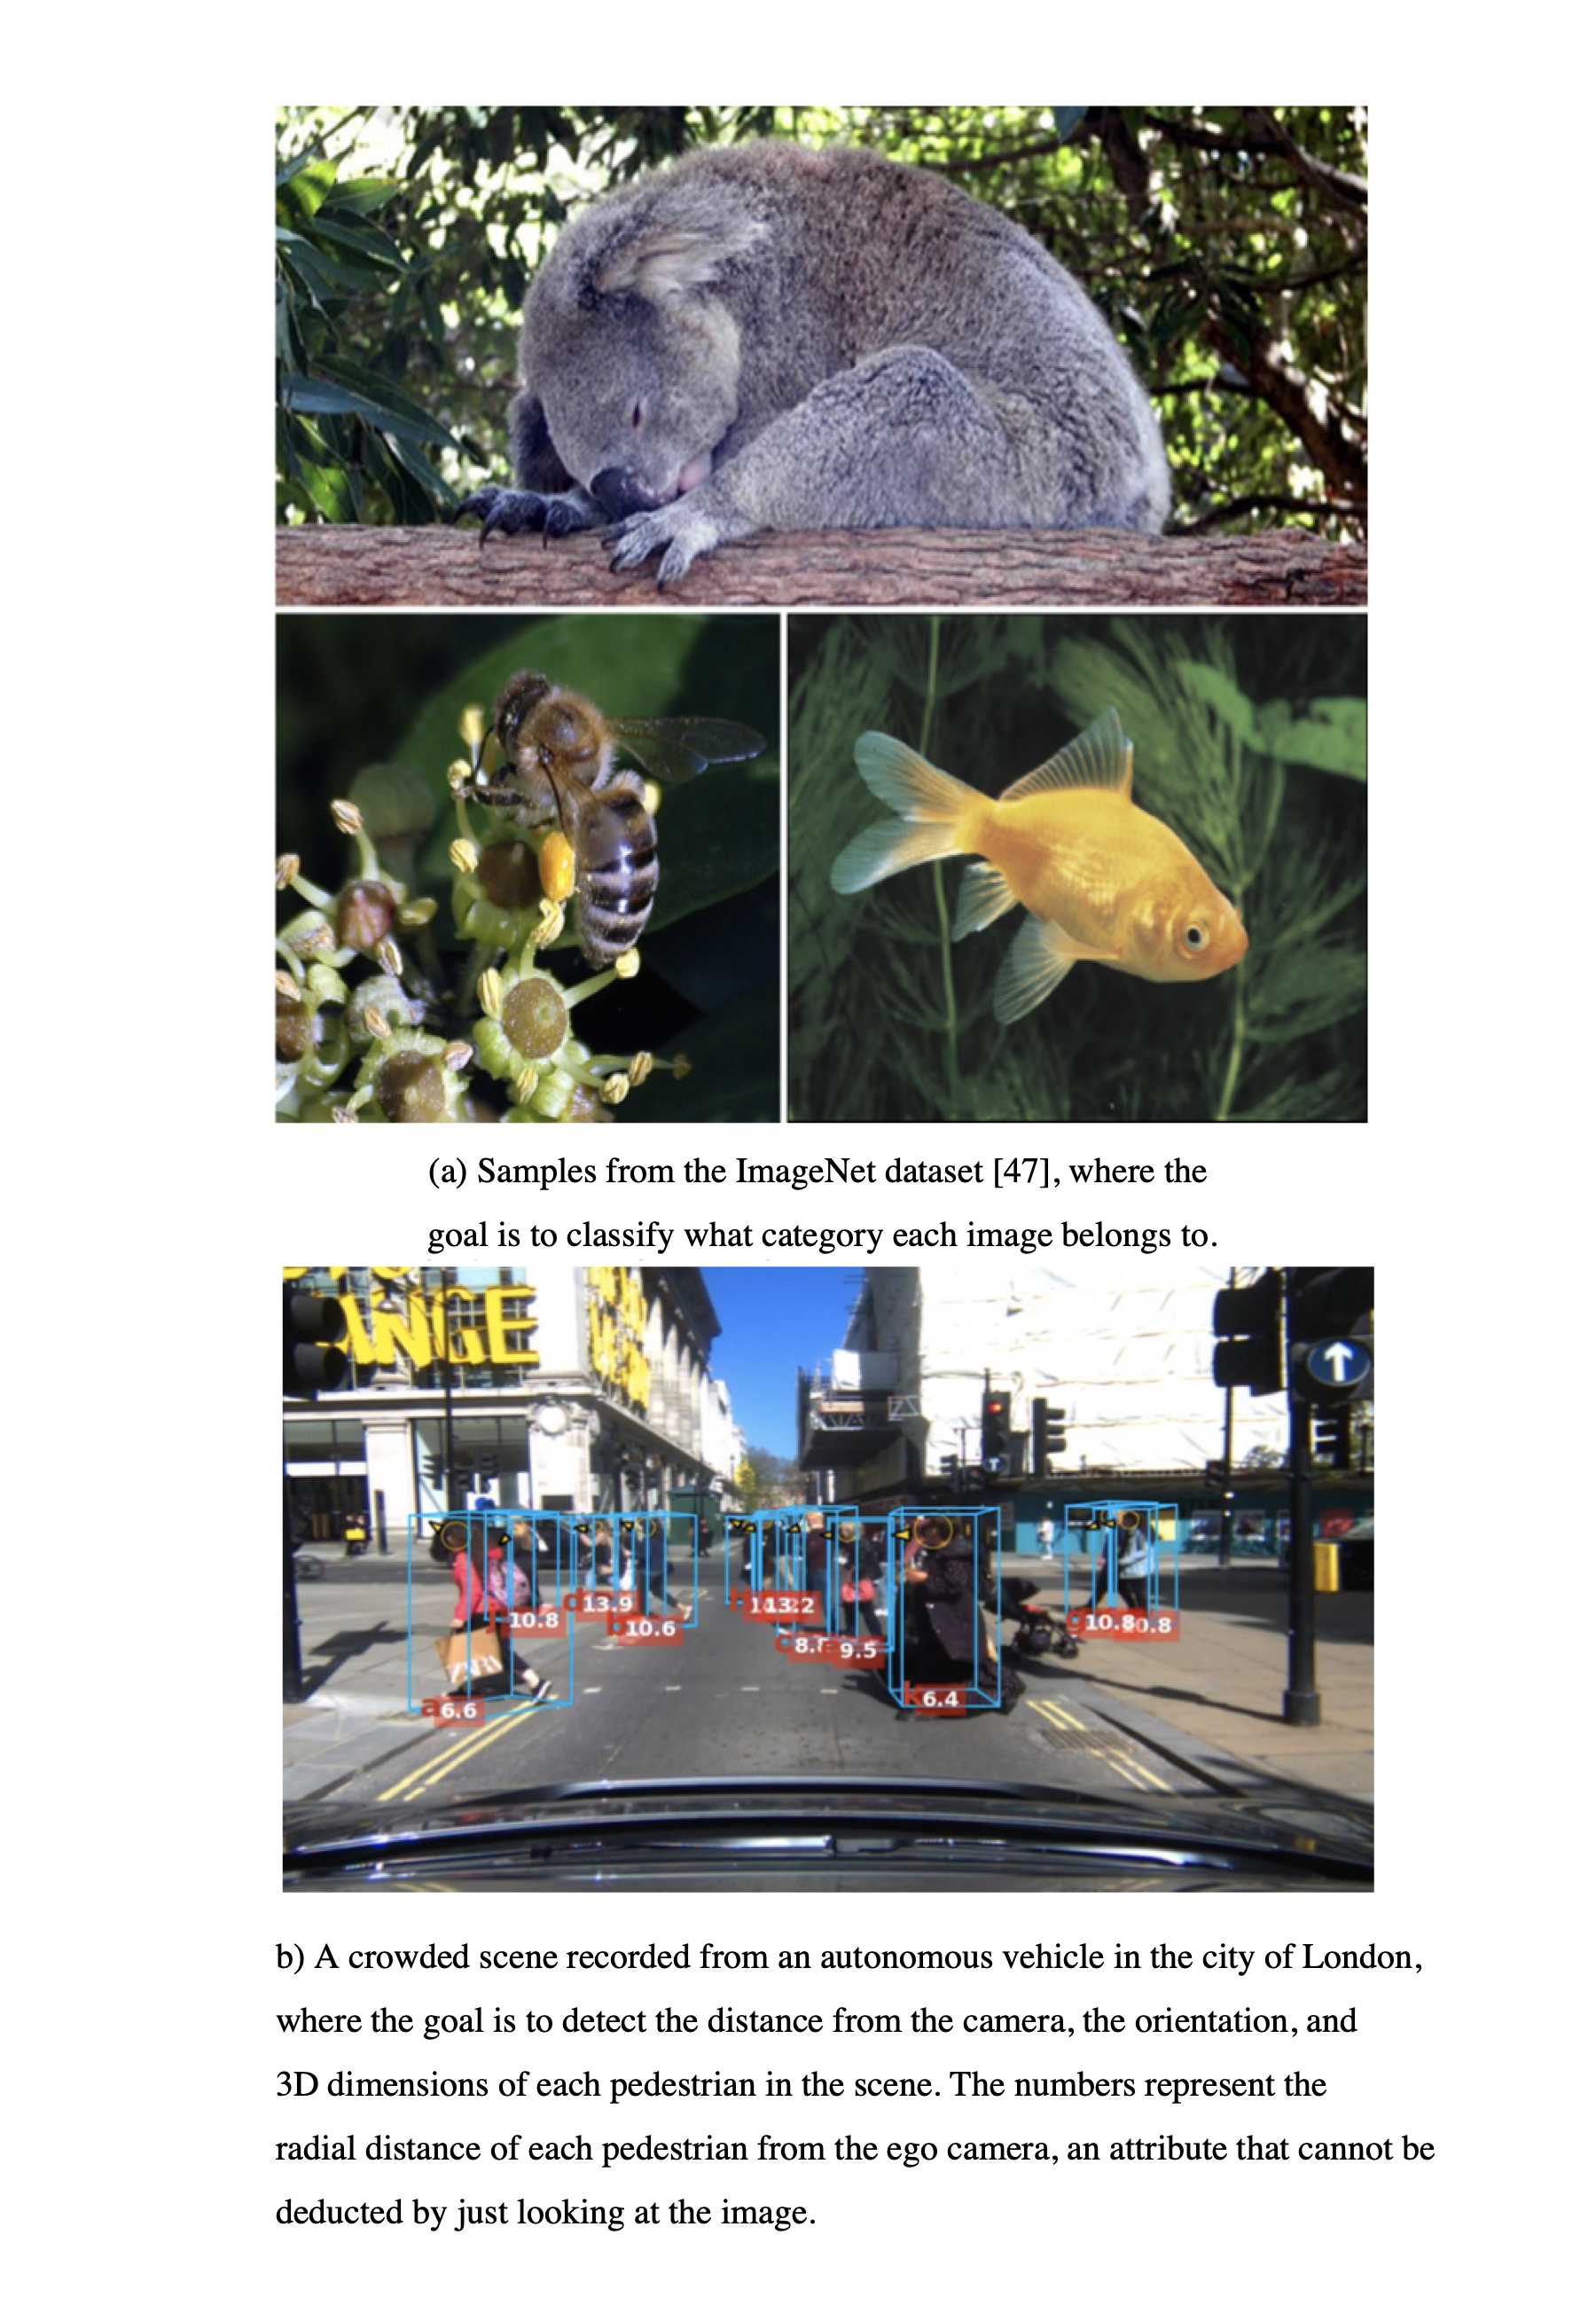
\includegraphics[width=\linewidth]{Images/int3.png}
    \caption{{Showing the evolution of computer vision tasks with deep learning; in this case, from 2D image classification (a) to 3D object detection (b).}}
    \label{fig:intro1 depth}
\end{figure}
 
In Figure \ref{fig:intro1 depth}, displays examples from the widely used ImageNet \cite{int17} dataset for image categorization and contrast them with a real-world image taken from an AV in London. In the first scenario, the image must be categorized in accordance with its class. In the latter scenario, the goal is 3D object detection, where each dynamic item is identified in 3D, i.e., the coordinates, orientation, and dimensions in the 3D world. Understanding the geometry of an object and its surroundings is particularly important for determining its 3D location (for example, is a car smaller or just farther away?). It can be difficult to recover 3D structures from projected images of moving objects or scenes, which presents difficulties not present in 2D perception tests. 
Deep learning algorithms that perceive the world in three dimensions, on the other hand, are typically trained on smaller datasets. The ImageNet collection has more than 14 million annotated photos, whereas KITTI \cite{int18}, the first dataset for 3D object detection, only has about 7500 images even though it was published four years after ImageNet. Since each object in the 3D scene needs to be labeled, annotating a 3D dataset takes more time and necessitates the use of specialized equipment like LiDARs to gather ground-truth data. In Figure \ref{fig:intro1 depth}a, the sorts of animals are clearly identifiable, but in Figure \ref{fig:intro1 depth}b, a human annotator cannot tell from the image how far away the people are from the camera. 
It is more difficult for 3D perception systems to compare favorably to 2D perception systems and to generalize effectively to circumstances that have not been observed because of the complexity of the 3D world and the high expense of 3D labeling. 





\section{Approach}

\lettrine[lines=2, findent=3pt, nindent=0pt]{D}{}epth estimation from stereo images is a fundamental problem in computer vision due to its numerous applications in areas such as robotics, self-driving vehicles, unmanned aerial vehicles (UAVs), virtual and augmented reality, and 3D model reconstruction. Given a pair of images, depth estimation aims to compute the disparity between each pixel in the reference image and its correspondence in the target image. Accurate depth estimation is critical for many tasks, including obstacle detection and avoidance, navigation, and scene understanding.

The traditional pipeline for stereo matching involves hand-crafted cost aggregation methods such as semi-global block-matching, and Markov random field-based techniques that combine pixel-wise predictions and local smoothness into an energy function. These approaches, while successful in some cases, have shown limitations when dealing with occlusion, repetitive patterns, textureless areas, reflective surfaces, and thin structures. These challenges arise more frequently in real-world scenarios, where the scene complexity and diversity are significantly higher than in controlled or synthetic environments.

Recent advancements in deep learning have led to the development of more efficient and accurate stereo depth estimation methods, which can learn powerful representations and adapt to varying scene conditions. These methods have significantly outperformed traditional hand-crafted approaches on a variety of benchmark datasets. However, most existing datasets for depth estimation, such as MP3D\cite{ref:d3} and SF3D\cite{ref:SF3D}, are synthetic in nature, which limits the applicability of the derived algorithms to real-world scenarios. Moreover, these datasets focus primarily on conventional stereo camera setups, which do not fully capture the complexity and richness of 360$^\circ$ images.  In contrast to LiDARs, cameras are already installed in a large number of vehicles, and they are orders of magnitude cheaper. If extracting 3D information from a single RGB image is a fundamentally ill-posed problem, there is no intrinsic limitation when using stereo cameras. However, vision-based 3D object detection algorithms are still lagging behind LiDAR ones \cite{int19,int20}. These results depend not only on the sensor quality, but they are also a consequence of data availability. In fact, many recent 3D vision datasets include in their sensor suite multiple expensive LiDARs while lacking a low-cost stereo camera \cite{int21 ,int22, int23}. We hope our research can contribute to revert this tendency towards a more balanced sensor suite.

\begin{figure}[h]
    \centering
    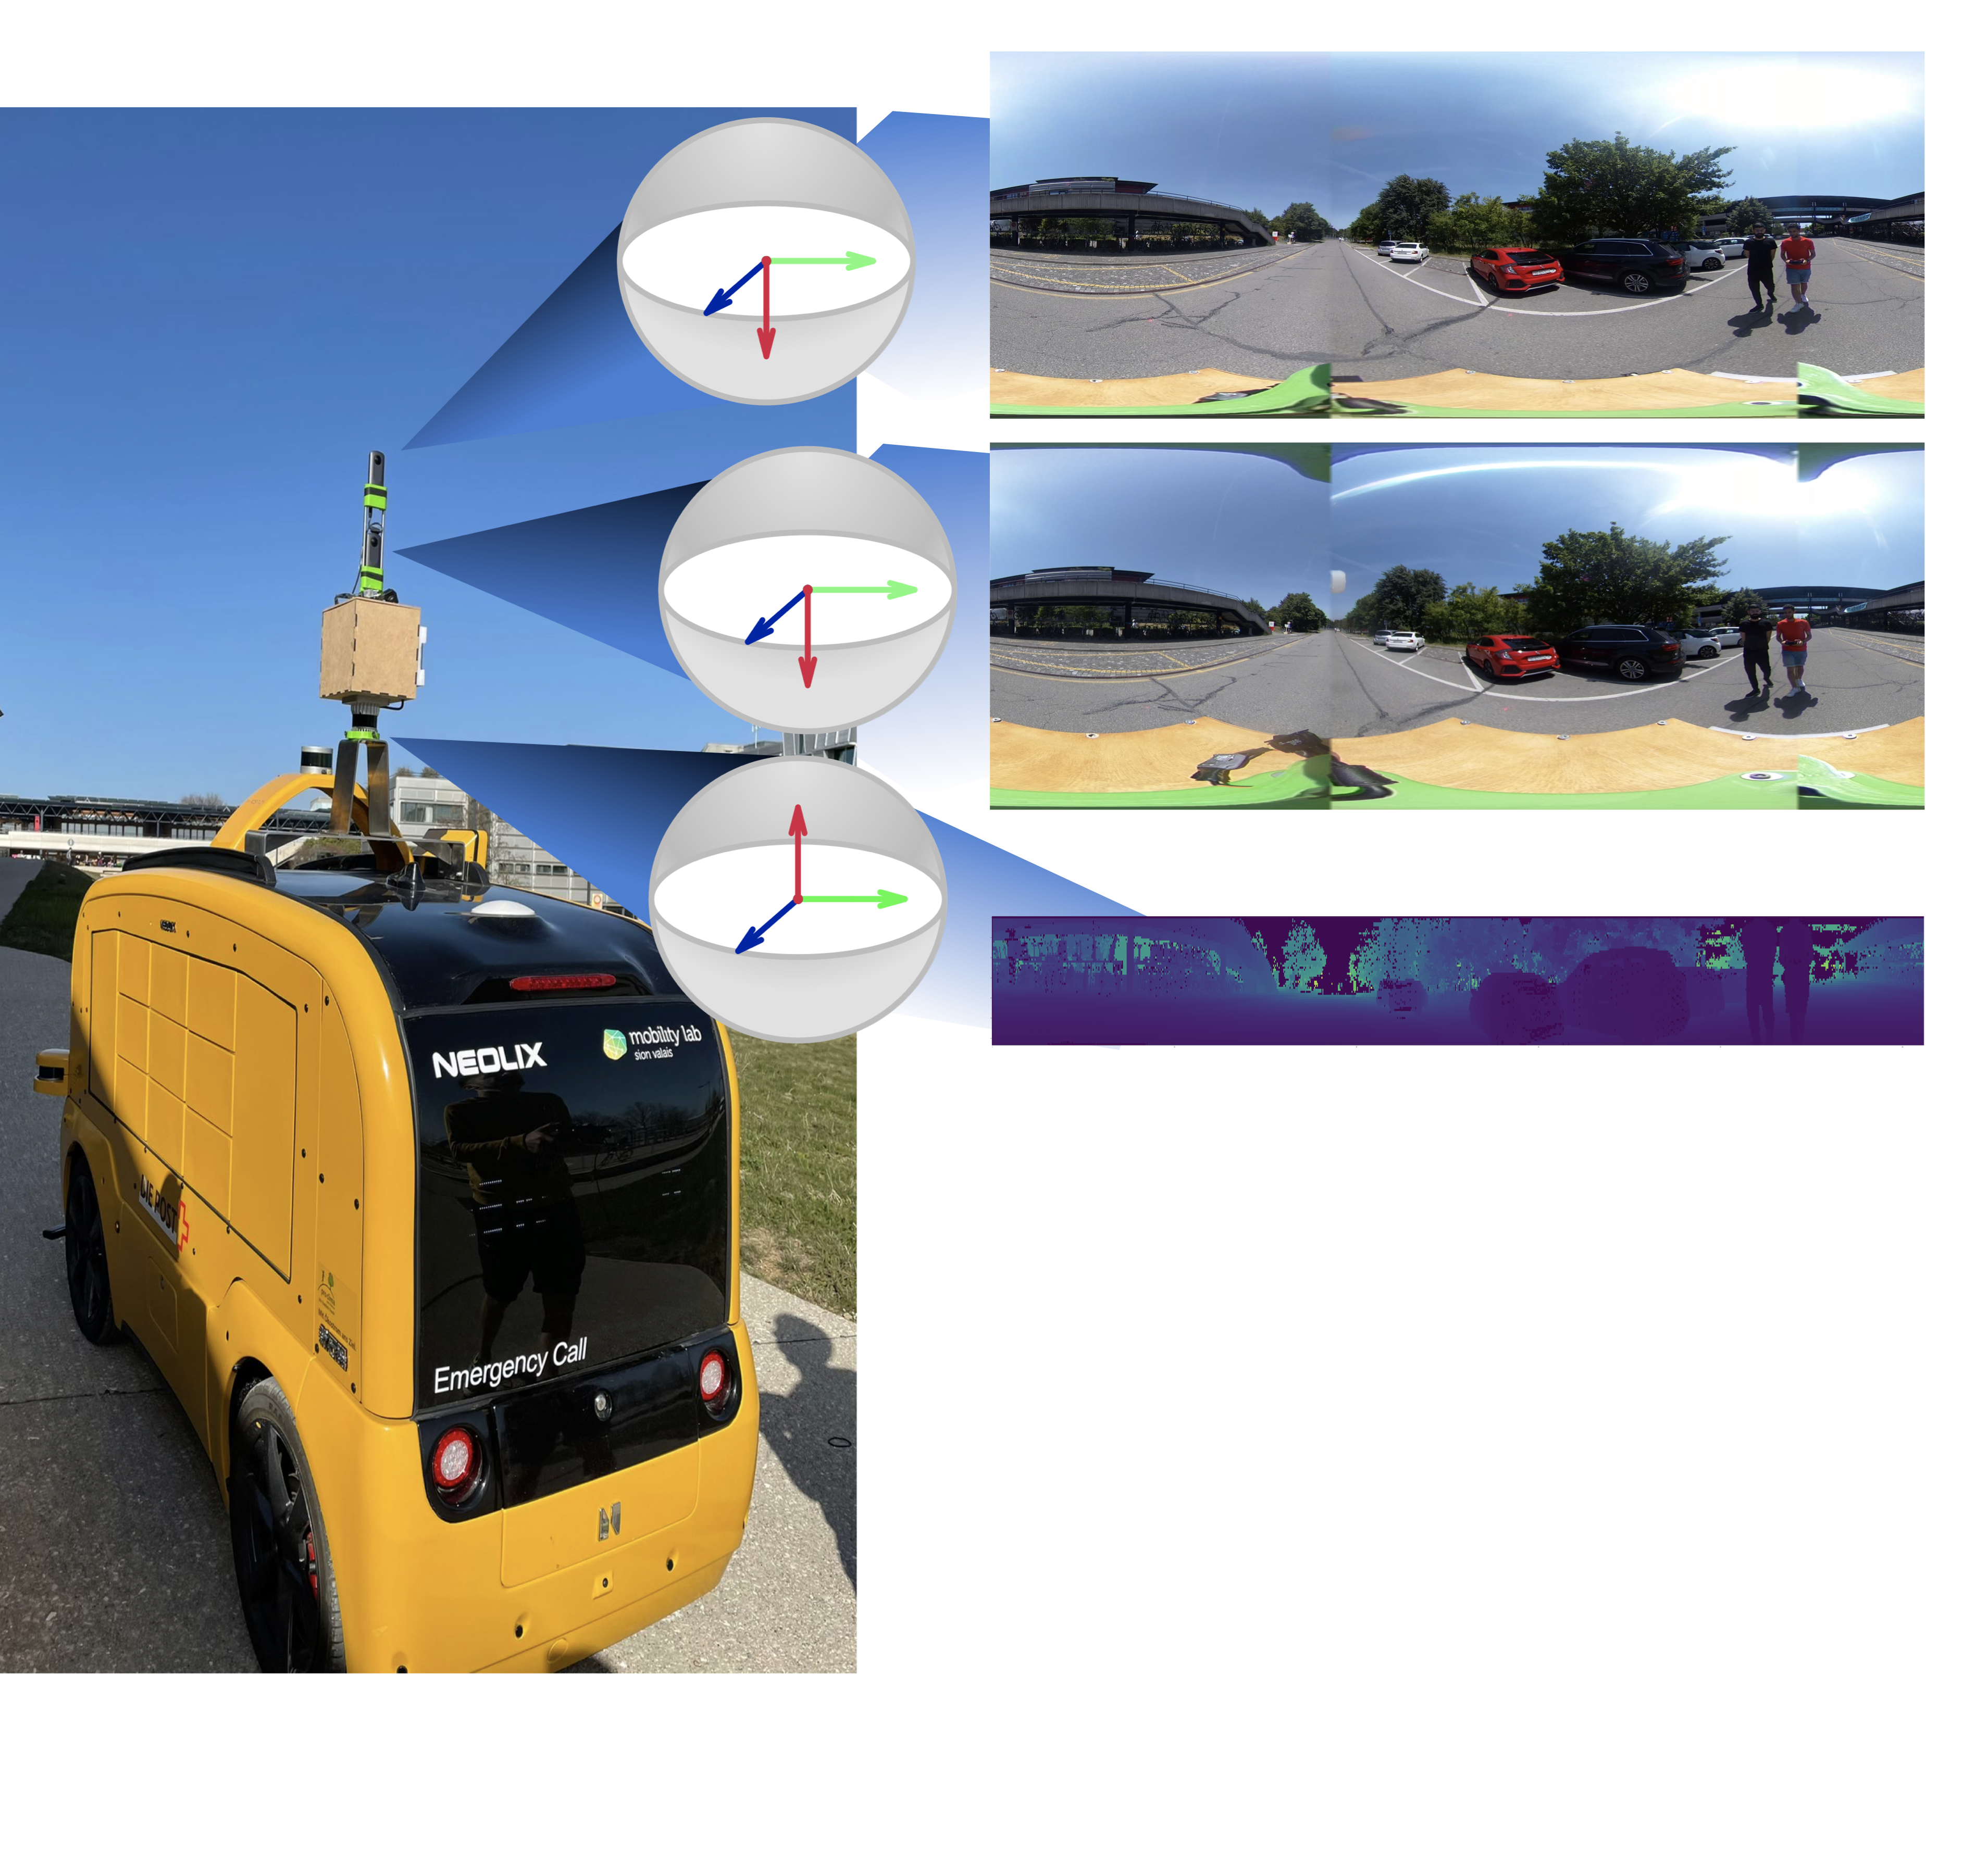
\includegraphics[width=\linewidth]{Images/21.png}
    \caption{\textbf{Dataset recording system.} A new dynamic dataset of real-world data containing stereo 360° cameras and LiDAR depth images.}
    \label{fig:21 depth}
\end{figure}

This thesis aims to address these limitations by introducing a new dataset for depth estimation from stereo 360-degree images and exploring the challenges and opportunities associated with it. Our dataset possesses several unique characteristics that set it apart from existing datasets:

\begin{enumerate}
    \item Real-world Images: Unlike synthetic datasets, our dataset consists of real-world images, which inherently contain more complex and diverse scene structures. This enables the development of algorithms that generalize better to real-world scenarios and enhances the robustness of the depth estimation process.
    \item Vertical Camera and LiDAR Setup: Our dataset employs a vertical setup for cameras and LiDAR sensors, which provides a more comprehensive understanding of the scene and captures information from different perspectives. This setup can potentially improve the accuracy and reliability of depth estimation in challenging environments Figure\ref{fig:21 depth}.
    \item Unrectified Image Pairs: The image pairs in our dataset are not rectified, meaning that they have not been preprocessed to align corresponding points along the same horizontal line. This introduces additional challenges to the depth estimation process, as the algorithms need to account for the disparity in image alignment while estimating depth.
    \item Depth Images as Ground-Truth: Instead of using disparity maps as ground-truth, our dataset provides depth images, which offer a more direct representation of the scene structure. This facilitates the evaluation of depth estimation algorithms and enables a more accurate comparison of their performance.
\end{enumerate}

In order to demonstrate the potential of our dataset, we evaluated the performance of popular depth estimation architectures, such as PSMNet and 360SD-Net, on our dataset. Through this process, we identified the strengths and weaknesses of these architectures in handling real-world, stereo 360-degree images. To further enhance the performance, we modified and added code to these architectures, ultimately proving that our dataset presents a new challenge for deep learning tasks in stereo depth estimation. By achieving satisfactory results at the primary level, we have laid the groundwork for future research in this area.



\section{Thesis Structure}
The remainder of this thesis is organized as follows:

\begin{itemize}
    \item \textbf{Chapter 2} provides a review of the related literature, focusing on the concept of depth estimation from pin-hole cameras and spherical cameras, as well as the state-of-the-art techniques in stereo depth estimation, traditional pipeline challenges, and the impact of deep learning in this field. Existing datasets for depth estimation and their limitations will also be discussed.
\item \textbf{Chapter 3} describes the proposed dataset in detail, explaining the process of data acquisition, the vertical camera and LiDAR setup, and the unique characteristics of the dataset. This chapter also discusses the generation of ground-truth depth images and the challenges introduced by the unrectified image pairs.
    \item \textbf{Chapter 4} delves into the architecture of deep learning-based depth estimation methods, specifically focusing on PSMNet and 360SD-Net. The different components and modules of these architectures will be explained, as well as the modifications and additions made to enhance their performance on our dataset.
    \item \textbf{Chapter 5} presents the experiments and results obtained by processing our dataset with various depth estimation architectures. This chapter will discuss the performance evaluation, comparisons with other methods, and insights gained from the experiments, highlighting the challenges and opportunities presented by our real-world stereo 360-degree image dataset.
    \item \textbf{Chapter 6} concludes the thesis by summarizing the main contributions, discussing the potential future research directions in the field of depth estimation from stereo 360-degree images, and reflecting on the implications of our findings for the broader field of computer vision.
\end{itemize}

By introducing a new dataset and evaluating the performance of existing depth estimation architectures on it, this thesis aims to contribute to the advancement of stereo depth estimation research and pave the way for future studies that further explore the challenges and opportunities associated with real-world, stereo 360-degree images.



% ################################## Chapter 2 #######################################
% ####################################################################################

% ################################################################################
\chapter{State of the art}
\label{chap:1} 

The stereo method is a relatively mature concept in computer vision, and the stereo method has been investigated in a number of studies. However, most of these studies used standard cameras with a limited FOV, and the analyses were based on the pinhole camera model. Image sensors can be divided into standard cameras with a narrow view and omnidirectional cameras with a much wide view. A camera with wide views means acquiring more information. The omnidirectional images are used widely in telepresence, 3D reconstruction, and autonomous robot navigation, such as obstacle avoidance. In addition a cylindrical image has a full 360-degree view along an azimuth angle; it is difficult to represent the scene on the top or the bottom of the camera sensors since the height of the cylindrical image would have an almost infinite value for these scene points. However, a spherical image may have a complete view. Realizing a spherical stereo means that the recovery of the surrounding structure of environments is possible more easily. It is necessary for some applications, such as constructing an immersive virtual environment \cite{ref:Spherical stereo, ref:Binocular spherical}.


\section{Pinhole Camera Model}
\label{sec:caso}
\newcommand\textsub[1]{\stackengine{-.5ex}{}{\scriptsize#1}{O}{l}{F}{F}{L}}

In computer vision, the most popular camera model is the pinhole camera model, in which the environment is perspectively projected onto a planar image, Consider the following problem: given two images taken from cameras at different horizontal/Vertical positions, the goal is to find depth for each pixel in pair of images. Despite many studies developed tons of approaches toward this issue, the primary approach has been proposed based on the simulating human binocular, by computation of disparity which is defined as the angle difference between the point of projection on the retina, which is part of the sphere rather than a plane similar to human vision\cite{ref:Spherical stereo}.
% \begin{figure}[h]
%     \centering
%     \includegraphics[scale=0.35]{Images/depth.png}
%     \caption{The stereo model of BSV.}
% \end{figure}

% \includegraphics[scale=0.35]{Images/depth.png}
The binocular stereo vision (BSV) depth estimation technology employs an anthropomorphic approach to perceive the depth of the surrounding environment and obtain three-dimensional information about real-world targets. The method uses two coplanar cameras, positioned parallel to each other, to capture the same scene from different viewpoints. Depth information is then recovered by calculating the parallax value between corresponding points in the image pairs, following the principle of triangulation. This approach utilizes the optical centers of the left and right cameras (O\textsub{l} and O\textsub{r}) along with their respective camera coordinate systems (O\textsub{l}\textendash X\textsub{l} Y\textsub{l} Z\textsub{l} and O\textsub{r}\textendash X\textsub{r} Y\textsub{r} Z\textsub{r})\cite{ref:s3}. The horizontal distance between the optical centers referred to as the baseline distance (b), and the focal length of the camera (f) are also considered in depth estimation. For a three-dimensional space point P(X, Y, Z), the projection point coordinates in the left and right imaging coordinate systems (p(x\textsub{l},y\textsub{l}) and p(x\textsub{r},y\textsub{r}), respectively) are used in triangulation to estimate its depth, a visual representation of this process is depicted in Figure \ref{fig:stereo depth}\cite{ref:s3}.

\begin{figure}[h]
    \centering
    \includegraphics[width=\linewidth]{Images/depth.png}
    \caption{The stereo model of BSV.}
    \label{fig:stereo depth}
\end{figure}



\begin{figure}[h]
    \centering
    \includegraphics[width=\linewidth]{Images/depth pinhole.png}
    \caption{Projection plane of BSV model to the XOZ plane.}
    \label{fig:XOZ}
\end{figure}

Consider Figure \ref{fig:XOZ}, based on the triangulation similarity principle:
\vspace{1cm}

\begin{align}
    \frac{z}{f} &= \frac{x}{x\textsubscript{l}} \\
    \frac{z}{f} &= \frac{x - b}{x\textsubscript{r}} \\
    \frac{z}{f} &= \frac{y}{y\textsubscript{l}} = \frac{y}{y\textsubscript{r}}
\end{align}

% \begin{equation}
% \begin{flalign*}
%          \frac{z}{f} = \frac{x}{x\textsub{l}}  \\
%          \frac{z}{f} = \frac{x - b}{x\textsub{r}} \\
%          \frac{z}{f} = \frac{y}{y\textsub{l}} = \frac{y}{y\textsub{r}}
%     \end{flalign*}
% \end{equation}

\vspace{1cm}

Then it can be received:
\begin{equation}\label{eq:2}
\begin{flalign*}
         z &= \frac{fb}{x\textsub{l} - x\textsub{r}} = \frac{fb}{d}  \\
         x &= \frac{x\textsub{l} \times z}{f}  \\
         y &= \frac{y\textsub{l} \times z}{f}  
    \end{flalign*}
\end{equation}

\vspace{1cm}



In  equation \ref{eq:2} the disparity would be defined as the offset of projection of point \emph P to the left and right camera planes which can be determined by \textit{x\textsub{l} - x\textsub{r}}; then \emph Z depth value of point \emph P can be determined from known values of parameters of f and b.

However, the conventional stereo planer cannot cope with wider field of view(FOV) as the pinhole camera model requires an image of infinite size to represent a FOV\cite{{ref:Binocular spherical}}.

\section{Spherical Camera Model}
\label{sec:caso}

A spherical image has a FOV. By taking advantage of 360$^\circ$ cameras for complete observation in an environment, the estimated depth from these cameras could be utilized for 3D reconstructing the entire surrounding. 

Assume a sphere with the characterization of radius f\textsub{s} and a point P in space as Figure \ref{fig:spherical plane}. Spherical projection is the intersection of the sphere surface with the line-intersecting point P, and the sphere's center. With this consideration, a spherical image can be derived by projecting all the visible points from the sphere. Thus spherical image includes part or the whole surface of a sphere\cite{ref:Binocular spherical,ref:Spherical stereo}. 

\begin{figure}[h]
    \centering
    \includegraphics[scale=0.7]{Images/spherical plane.png}
    \caption{ Spherical projection based on a spherical camera model.}
    \label{fig:spherical plane}
\end{figure}

As the camera coordinate system is set at the center of a sphere, the ray direction of projection is determined by a polar angle $\theta$ and an azimuth angle, $\phi$. Suppose the coordinates (relative to the spherical image coordinate system) of a point P in space is 

\begin{equation}\label{eq:3}
\begin{flalign*}
         M_c = [X_c \quad Y_c \quad Z_c]^T
    \end{flalign*}
\end{equation}

\vspace{0.8cm}

then the projection of the point, p, in a spherical image can be represented as

\begin{equation}\label{eq:4}
\begin{flalign*}
         m = [f_s \sin \theta \cos \phi \quad f_s \sin \theta \sin \phi \quad f_s \cos \theta]^T
    \end{flalign*}
\end{equation}

\vspace{0.8cm}

then the relation between coordinate and projection is

\begin{equation}\label{eq:5}
\begin{flalign*}
         m = \lambda M \cong M_c
    \end{flalign*}
\end{equation}

\vspace{0.8cm}

where $\lambda = \frac{f_s}{\rho}$, and $\rho = \sqrt{{X_c}^2 + {Y_c}^2 + {Z_c}^2}$.
This means that m is equal with $M_c$ multiplied by a scale factor $f_s$\cite{ref:Binocular spherical,ref:Spherical stereo}. 

Letting $f_s = 1$ the normalized spherical image coordinates are then derived which corresponds to the projection onto a unit sphere.

Concerning the perspective projection of a planar image based upon a pin-hole camera model, a spherical projection has the following characteristics\cite{ref:Binocular spherical,ref:Spherical stereo}.
\begin{itemize}
  \item In a planar image, the projection of a scene point is represented by the coordinates of an image plane. This representation has the effect that every point in space, so long as it can be seen from the spherical view, can be equally represented in a spherical projection.
  \item The coordinate system of a spherical image is the same as the camera coordinate system.
  \item There is no specific optical axis employed as in the case of classical perspective projection because every ray from the environment that points to the spherical picture is perpendicular to the spherical surface.
  
\end{itemize}

\section{Disparity Definition of Spherical Stereo Camera}
\label{sec:Spherical disparity}

Imagine a set of two spherical cameras that capture images using spherical projection. Assume that the camera coordinate systems' axes are parallel to each other, and the x-axes are aligned in a straight line, as illustrated in Figure \ref{fig:spherical stereo}. The baseline of this spherical stereo setup is represented by the line connecting the two focal points. The epipoles in each spherical image are the points where the baseline intersects the image on the x-axis, and can be represented as (±1, 0, 0) in normalized spherical image coordinates. Epipolar lines are considered great circles, which are defined as the circles formed when a plane passing through the sphere's center intersects the sphere\cite{ref:Binocular spherical,ref:Spherical stereo}.


\begin{figure}[h]
    \centering
    \includegraphics[width=\linewidth]{Images/spherical.png}
    \caption{ Spherical stereo. A point is observed by a pair of spherical cameras.}
    \label{fig:spherical stereo}
\end{figure}



In our exploration of spherical stereo depth estimation, we examine the disparity within an epipolar plane, determined by a point in the environment and the two focal points, as illustrated in figure \ref{fig:disparity of spherical stereo}. Let the angles formed by the projection of point P onto the spherical images and the x-axis be denoted as ${\theta}_l$ (polar angle relative to the x-axis) and ${\theta}_r$, respectively. We define the disparity, $d_s$, of point P as the difference between the arc lengths $\alpha_l$ and $\alpha_r$, which are subtended by the angles ${\theta}_l$ and ${\theta}_r$, respectively. In the other word, 

\begin{equation}\label{eq:6}
\begin{flalign*}
         d_s = $\alpha_l$ - $\alpha_r$ = f_s($\theta_l$ - \theta_r)
    \end{flalign*}
\end{equation}

notice that in equation \ref{eq:6} $f_s$ represents the radius of the great circle which is the focal length of the spherical image. 

\begin{figure}[h]
    \centering
    \includegraphics[width=0.9\linewidth, height=8cm]{Images/s2s(1).png}
    \caption{ Definition of disparity for spherical stereo.}
    \label{fig:disparity of spherical stereo}
\end{figure}


we consider a normalized spherical image with a focal length $f_s$ of 1. The normalized disparity $d_n$ in a spherical stereo system can be determined by the difference between the angles ${\theta}_l$ and ${\theta}_r$, i.e

\begin{equation}\label{eq:7}
\begin{flalign*}
         d_n = $\theta_l$ - \theta_r
    \end{flalign*}
\end{equation}

The concept of normalized disparity, is denoted as $d_n$. This disparity is associated with the angle $\angle P$, which is formed by the rays originating from point P and extending to the focal points of the pair of spherical images. Importantly, this measure of disparity is independent of the intrinsic parameters of the spherical cameras. The term "spherical disparity" is used to differentiate this concept from the traditional disparity observed in planar stereo images.

\section{Computing Distance of observed Points in environment}
\label{sec:Computing Distance of observed Points in environment}

 the point location in space is defined by the distance within the spherical stereo, rather than the depth conventionally used in planar stereo. This is because environment points are equally represented in spherical images, and due to the lack of an optical axis in these images, all projection rays are perpendicular to the spherical image. Consequently, the position of a point in space is described by its distance from the center of the gravity of the sphere. Considering the arcs $\alpha_l$ and $\alpha_r$ subtended by angles $\theta_l$ and $\theta_r$, respectively, the distances of point P from the two spherical cameras can be determined using the sine theorem \cite{ref:Binocular spherical,ref:Spherical stereo},
 \begin{equation}\label{eq:8}
\begin{flalign*}
         \rho_l = b_s \frac{sin\theta_r}{\sin \theta_l - \sin\theta_r} = b_s \frac{\sin \frac{\alpha_r}{f_s}}{\sin(\frac{\alpha_l}{f_s} - \frac{\alpha_r}{f_s})} =  b_s \frac{\sin \frac{\alpha_r}{f_s}}{\sin(\frac{d_s}{f_s})}
    \end{flalign*}
\end{equation}

\begin{equation}\label{eq:9}
\begin{flalign*}
         \rho_r = b_s \frac{sin (\pi - \theta_r)}{\sin \theta_l - \sin\theta_r} = b_s \frac{\sin (\pi - \frac{\alpha_r}{f_s})}{\sin(\frac{\alpha_l}{f_s} - \frac{\alpha_r}{f_s})} =  b_s \frac{\sin(\pi -  \frac{\alpha_r}{f_s})}{\sin(\frac{d_s}{f_s})}
    \end{flalign*}
\end{equation}

respectively, where $\theta_l$ and $\theta_r$ can simply be computed from the spherical image coordinates of the projection.


\section{ Latitude-longitude presentation}

In the field of spherical stereo images, latitude-longitude geometry offers an alternative way to represent these Figures \ref{fig:cy}. This method arranges the great circles, which intersect at the epipoles, into parallel straight lines\cite{f1}. As a result, conventional correlation-based matching techniques with a 1D search range can be employed to calculate the disparity of spherical stereo images, as long as they are vertically aligned \cite{f2}.

It is essential to ensure that the displacement between the camera views remains parallel to the direction of the line scan camera pixel array. This alignment causes the epipolar lines to correspond to pixel columns in the spherical images \cite{f3}. The accuracy of this method relies on the mechanical precision of the line scan camera. However, if a less accurate camera system is used, rectification can be employed to correct errors to some extent \cite{f2}.


\begin{figure}[h]
    \centering
    \includegraphics[width=\linewidth]{Images/cy1.png}
    \caption{Spherical image representation: (a)Spherical imaging; (b)Latitude-longitude imaging.}
    \label{fig:cy}
\end{figure}
% ################################# End Chapter 2 ###################################

% ################################## Chapter 3 #####################################
% ##################################################################################
\chapter{Dataset}
\label{chap:2}
\section{Dataset Overview}

The dataset has been collected in four different locations. We provide two collections in two wide-ranging outdoor street areas and two indoor corridors. The two indoor scenes have been made in an educational institution around offices in \textit{École Polytechnique Fédérale de Lausanne} (EPFL). 
For each recorded scene, the dataset is constituted of 3 different parts: upper camera images, lower camera images, and the corresponding LiDAR depth images along with point clouds.
Thus, our proposed dataset comes in a 3-tuples list where an image in one folder of some index is linked to the same index in the two other folders. 
The stereo images consist of high-resolution images with 3840 in width and 1920 in height. The depth images have a resolution of 1024 in width and 64 in height. The small resolution of depth images is related to our Lidar (Ouster OS1-64) limitation, which has a maximum resolution of 64 in height\cite{ref:ouster}.
Our design involves vertical camera displacement similar to that in\cite{c18, c19, c20}. Therefore, all pixel displacements on the spherical picture will align with the equirectangular image's vertical lines. All of the previous literature devoted some efforts to calibrating the top and bottom images by implying rectification toolboxes(Kailibr), thus disparity estimation is made much easier by searching within the same vertical line on the equirectangular images. More specifically, \cite{c21} experiments show interior/relative orientation parameters for camera RICOH Theta which we have used for extracting our dataset. However, we make the choice not to rectify our dataset. This approach makes the learning algorithm more difficult while helping to have a more generic dataset. Compared to other known 360 datasets \cite{c23}, the other advantage of our dataset is that it is composed of images from real and time-synchronized scenes. In contrast, the others consist of synthetic images. The resulting dataset corresponds to a total of 17'373 tuples that can be reconverted into synchronized videos back again.

\begin{table}[!h]
\caption{Information and Cardinality of Data}
\label{table_example}
\begin{center}
\begin{tabular}{|c||c||c||c|}
\hline
Dataset & Type of Data & Cardinality\\
\hline
Outdoor1 & Real & 7669\\
\hline
Outdoor2 & Real & 3333\\
\hline
Indoor1 & Real & 2121 \\
\hline
Indoor2 & Real & 4250 \\
\hline
\end{tabular}
\end{center}
\end{table}

\section{Related datasets}
Several relevant datasets have been developed in the context of depth estimation from 360$^\circ$ images, providing valuable resources for researchers in computer vision, scene understanding, and 3D reconstruction. These datasets vary in data acquisition techniques, size, and scope, catering to a range of depth estimation tasks. In this discussion, we focus on the KITTI dataset, SceneFlow dataset, Matterport3D (MP3D), and Stanford 3D Scanning Repository (SF3D), comparing their strengths and limitations\cite{ref:d1}\cite{ref:d2} \cite{ref:d3}\cite{ref:SF3D}.
The KITTI and SceneFlow datasets cater to outdoor and synthetic scenarios, respectively, both providing rectified stereo images and ground truth depth maps. The KITTI dataset, a comprehensive benchmark suite, primarily targets computer vision tasks in autonomous driving applications, offering real-world scenarios captured in complex urban and rural environments. In contrast, the SceneFlow dataset, a large-scale synthetic dataset, is designed specifically for optical flow and disparity estimation, allowing researchers to assess the performance of their methods under diverse and controlled conditions.
Focusing on indoor scenes and 3D reconstructions, the Matterport3D and Stanford 3D Scanning Repository datasets offer unique perspectives. The MP3D dataset comprises real-world indoor panoramic images, captured using the Matterport Pro 3D camera, which performs on-device depth rectification. This dataset is particularly suitable for depth estimation from 360$^\circ$ images, providing panoramic views with corresponding depth maps and surface normal information. Conversely, the SF3D dataset is a collection of 3D models obtained by scanning real-world objects and scenes, utilizing a volumetric method for building complex models from range images. While not explicitly targeting depth estimation from 360$^\circ$ images, it remains a valuable resource for benchmarking 3D reconstruction, mesh processing, and computer graphics algorithms.
The KITTI and SceneFlow datasets offer insights into various outdoor and synthetic scenarios, while the Matterport3D dataset caters to real-world indoor panoramic views with depth information. The SF3D dataset, although not directly targeting depth estimation from 360$^\circ$ images, provides 3D models from scanned objects and scenes for related computer vision tasks. When leveraged effectively, these diverse datasets can significantly contribute to advancements in depth estimation from 360$^\circ$ images.




\section{Dataset Characteristics and Format}
One challenging task when recording data from different kinds of devices is the output format that usually does not match, which could be hard for learning tasks afterward. In our dataset, we overcome this challenge by removing the LiDAR distortion and aligning it with the camera's format.

\begin{itemize}
  \item{\textbf{Camera Output:}}
Ricoh Theta is an omnidirectional camera resulting in a spherical output that can be accessed with special software (for VR navigation for instance). Obviously, the images can still be accessed with a simple image viewer and the data would then be projected on a 2D sub-space which leads to have severe Barrel distortion. 

    \item{\textbf{LiDAR Output:}}
LiDAR OS1 detects and generates point clouds representing depth all around the device. Thus the output is in a panoramic form with a vertical angle of 24°.

    \item{\textbf{Data Processing and Distortion Removal:}}
As mentioned, the cameras and LiDAR do not have the same data format but still, both can be interpreted as fixed frame images. 
The open-source driver outputs these data layers as fixed resolution 360° panoramic frames. This results in camera-like images.
A problem remaining is the image form, cameras are spherical while LiDAR depth images are panoramic. By definition, LiDAR's field of view is a "subset" of the camera one. Thus, to overcome this incompatibility, we can remove camera distortion in the poles and isolate the target part of the picture overlapping with the LiDAR frames.

\end{itemize}
In our dataset we provide original camera images along with tools to perform distortion removals to match LiDAR depth images.

\begin{figure}[h] %this figure will be at the right
    \centering
    \includegraphics[width=\linewidth]{Images/clear distorsion.png}
    \caption{Data Processing results}
    \label{fig:dataprocessing}
\end{figure}

\subsection{Devices synchronization}



Making the recordings synchronized is an important task to get done properly to get reliable data. This task is enough challenging that no dynamic stereo 360° dataset exists before ours. Indeed we propose two methods to fix synchronization; to provide and allow the community collects dynamic-synchronized real-world data.

\subsubsection{Real-Time synchronization} 

The best solution to real-time synchronize devices with OS1 LiDAR is to use ROS given the libraries provided by the company.
The Robot Operating System (ROS) is a set of software libraries and tools that help you build robot applications.
The provided Ricoh cameras film at a rate of 30 fps, the LiDAR at maximum 15 fps. 
Hence we created three ROS topics that publish their info (frames). Our synchronization function waits for the lowest frequency device to publish its info in order to catch the frames. Such a choice ensures us on taking the frames only when the three publishers provide data at "the same time" (ROS time) with a certain margin of the threshold.

\begin{figure}[h] %this figure will be at the right
    \centering
    \includegraphics[width=\linewidth]{Images/ros framework.png}
    \caption{ROS Architecture for synchronization}
    \label{fig:ros}
\end{figure}

However, further efforts are required for real-time synchronization. This discussed naive-based pipeline results in chaotic behavior as follows :

\begin{figure}[h] %this figure will be at the right
    \centering
    \includegraphics[width=\linewidth]{Images/trasnmitting delays.png}
    \caption{Ros Timestamp with arrival devices time}
    \label{fig:strangeb}
\end{figure}
    
This behavior is in fact due to the difference between the generation time of the frames and arrival time to the disk. Only high-end global shutter cameras could benefit from this solution as their generation time is constant and the transferring time to the disk can then be measured.

\subsubsection{Post recording synchronization} 
This solution is highly inspired by cinema movie slate. The process goes as follows \\
Record independently with the two cameras and LiDAR simultaneously and at some point activate the "slate".
The slate has two main parts, the camera's slate, and LiDAR slate.
Once activated the slate is represented by a powerful flash sign that's activated for (33ms: cameras fps) to dazzle cameras lenses at a single frame. At the same instant, it also saves the ROS timing of the LiDAR (at a nanosecond order).\\
As a result, once the videos are exported we identify the dazzled frames of the cameras and construct a new timestamp with these moments as a new start. We do the same thing with LiDAR.
Once done, we filter the synchronized data by only keeping the mod3 frames of the cameras to achieve the same amount of frames in the cameras and LiDAR ( cameras and LiDAR have 30fps and 10fps). This results in perfect synchronized data with a maximum delay of 15ms (maximum achievable with Ricoh Theta). \\

\subsection{Hardware Setup Configuration}
Collecting data with several devices requires lenses to be relatively placed at the same distances between each other. A solution for this task is to assemble a physical device that holds them all together as we suggest in our recording system.

\subsubsection{Devices Support} \
\newline
\begin{figure}[h] %this figure will be at the right
    \centering
    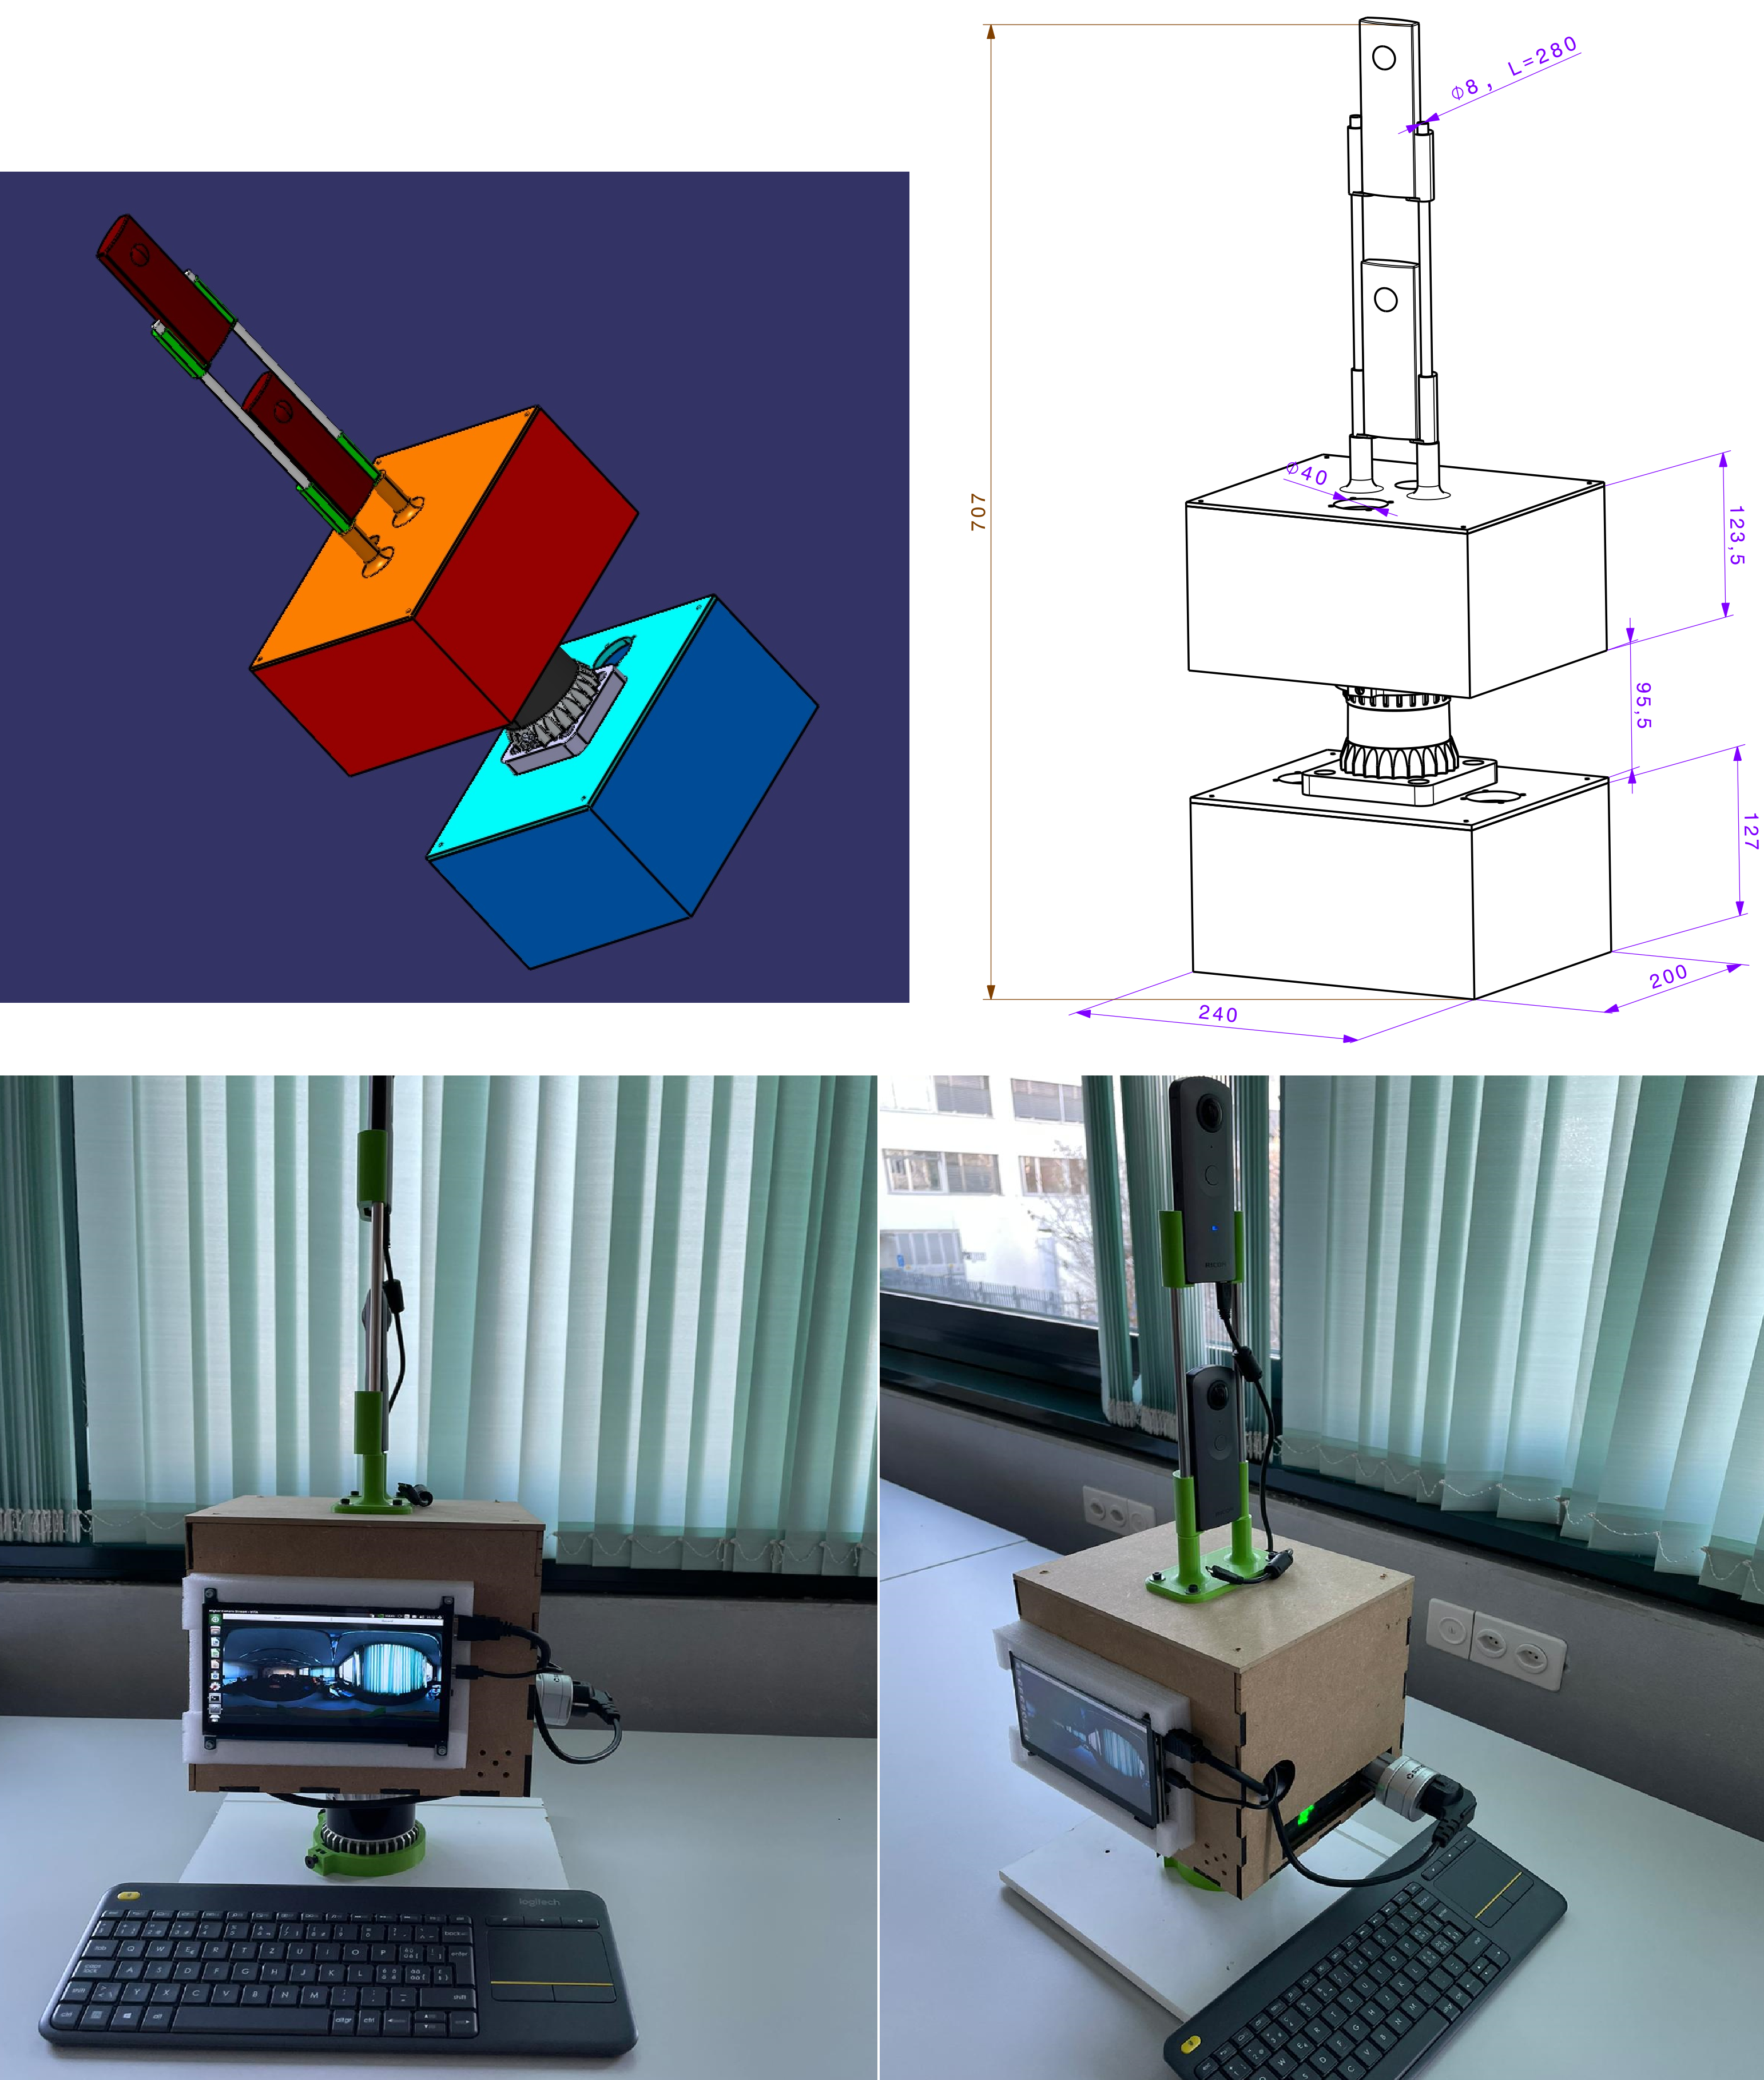
\includegraphics[scale=0.2]{Images/full architecture.png}
    \caption{Devices support prototype architecture}
    \label{fig:strangeb}
\end{figure}


The first support places the cameras horizontally at the first stage to test the behavior of the two cameras recording simultaneously.
But mainly to catch the perfect horizontal distance between them to have a good stereo without any distortions.
This can cause a problem as we are willing to do a stereo system with 360° cameras, and both must not see each other at the same time.
The first discovery was to find that putting the two cameras stuck together resolves the problem thanks to a blind spot of the cameras at a 180° angle, which makes the issue resolved.\\
The second part involves adding the LiDAR on the top or bottom of the support. In the meantime, we notice that horizontal stereo may cause depth detection problems as they won't have the same horizontal distances from objects as the LiDAR. 
Hence, we decided to improve the support as follows, making the stereo system going vertical.
Such a system is more reliable, as all the sensors are becoming aligned along the vertical axis.




These two boxes in this figure are made to hold the two computers on board (an Ubuntu computer for the cameras and another one for the LiDAR) along with their batteries to have a full on-board and movable system.\\
However, tests show that we need to have synchronization, which makes us use only one device to have all the information to synchronize in real time, which makes us switch to this final model, holding only one computer.

\subsubsection{Remotely Controlled Robot} \

% \begin{figure}[t] %this figure will be at the right
%     \centering
%     \includegraphics[width=120]{Images/loomo prototype.png}
%     \caption{Remotely controlled robot architecture}
%     \label{fig:strangeb}
% \end{figure}


\begin{figure*}[h!] %this figure will be at the right
    \centering
    \includegraphics[width=\linewidth]{Images/c1.jpeg}
    \caption{Dataset frame overview}
    \label{fig:l}
\end{figure*}

A simple 4-channel remote controller is used for controlling the motion of the robot, using the two vertical axes on the remote control to control the speed and direction of the robot’s wheels. The signal yielded by the receiver is a PWM signal that goes directly to the H-bridge motor driver which allows control of the rotation direction of the motors. There are 4 channels, each motor uses 2 channels for the forward and backward speeds.

\subsection{Dataset}
We perform our experiments on Outdoor1 and Outdoor2 datasets. The configuration of our dataset is a pair of $360^\circ$ top-bottom \textit{not rectified} images with equirectangular projection. The distortion in an image mainly includes textureless regions of images which are consisted of the sky and part of the setup in the top and bottom, respectively. The resolution of our images after distortion removal is 256 in height and 1024 in width. Furthermore, during training, we decided to crop images into 256 in height and 256 in width in order to reduce the number of computations in matching cost. 
\newpage
An example of our data without distortion removal is shown in figure \ref{fig:l}.
% The distribution of our Outdoor1 dataset for training and validation is 613/144, and for Outdoor1/Outdoor2 is 880/211. As our dataset is collected from a video and based on the synchronization, we have ten images per second, we decided to use only one fps in our training. 

\section{Rectification}
Stereo 360-degree images rectification is an essential preprocessing step in many computer vision applications such as 3D reconstruction, depth estimation, and object detection in panoramic images. The process involves transforming stereo images so that the corresponding points between the left and right images lie on the same horizontal line, simplifying the subsequent steps in stereo matching and disparity computation.

The Ricoh Theta is one of the cameras for capturing 360$^\circ$ images. In a paper by Aghayari S. et al. (2017)\cite{ref:rectification1}, the authors proposed a method for geometric calibration of full spherical panoramic Ricoh Theta cameras. They introduced an approach that models the camera as a pair of fisheye lenses. They also derived a mathematical model from mapping the spherical coordinates of points in 3D space to pixel coordinates in the equirectangular image. The calibration process involves estimating the intrinsic and extrinsic parameters of the camera, which are then used to rectify the stereo images.

It was mentioned as Ricoh-Theta camera consists of two lenses: front and back lens, and respective captured images are called central and side images here. These images are stitched together to form a full spherical image. Calibration procedure of each lens is performed separately and it starts by defining three spaces as follows: 1- Image space 2- Unit sphere space 3- Object space Calibration procedures perform in both unit sphere space for interior orientation parameters (IOPs) and object space for relative orientation parameters (ROPs). It means that image coordinates are first moved to unit sphere by equirectangular projection to be converted to spherical coordinate system. Furthermore, 3D points in the object space are moved to unit sphere by applying Helmert transformation (three translations and three rotations) between world and unit sphere coordinates. Therefore, 2D and 3D points from image space and object space are projected to unit sphere. Following this,, IOPs and EOPs are obtained by applying a rigorous statistical bundle adjustment procedure. The final step is the computation of ROPs from calculated EOPs of two lenses. 

Another significant contribution to stereo rectification for equirectangular images is Ohashi, Akira, et al. (2017) work \cite{ref:rectification2}. The authors proposed a novel method for rectifying stereo pairs of equirectangular images generated from a 360-degree camera. Their approach is based on the computation of an optimal rectifying homography, which minimizes the epipolar error. The method is effective in correcting geometric distortions, such as radial and tangential distortions, commonly found in fisheye lenses.

Fusiello, Andrea, Emanuele Trucco, and Alessandro Verri (2000) introduced a compact algorithm for rectifying stereo pairs, which applies to both traditional and equirectangular images\cite{ref:rectification3}. The algorithm is based on a projective transformation that maps the original images onto a common plane, where the corresponding points share the same horizontal coordinate. The method is computationally efficient and has been widely adopted in various computer vision applications.
However, in order to have the most robust model disregard the type of data, our dataset is not rectified. This decision was taken to tackle the depth estimation issue in all kinds of data. 


\vspace{1cm}
In order to show that our data is not rectified, the disparityMap function included in Matlab has been used, which computes the disparity map through semi-global matching, and the figure \ref{fig:kitti_disp} shows it can ideally compute the disparity map of the KITTI dataset, which its disparity is horizontal. As the function computes the disparity horizontally, it is needed to rotate 90$^{\circ}$ the images with vertical disparity, such as the MP3D dataset and ours. The result of the disparity map of MP3D is shown in the figure \ref{fig:mp3d_disp}. Finally, by following the same steps as MP3D, the disparity map of our data is shown in the figure \ref{fig:ours}. This approves that our data is not rectified. 

rectification is an essential preprocessing step for stereo vision algorithms. It aligns images in a stereo pair horizontally, simplifying the depth estimation process and improving model performance. Utilizing a non-rectified dataset can lead to reduced accuracy, slower convergence, and decreased robustness due to inconsistencies in image pairs and the propagation of camera calibration errors and lens distortions. Moreover, non-rectified datasets can negatively impact the efficiency of the depth estimation algorithms, as they require more computational resources to search for matching points in non-aligned images.

Rectified datasets, on the other hand, facilitate faster convergence and improve the interpretability of the model's output. They provide cleaner and more consistent inputs, making it easier to analyze the performance of the depth estimation model and identify potential issues. In conclusion, using a non-rectified dataset for depth estimation can result in several limitations, including reduced accuracy, robustness, and interpretability, as well as increased computational requirements. Therefore, it is crucial to rectify the dataset before employing it for depth estimation tasks in deep learning.
\vspace{0.9cm}

\begin{figure*}[h] %this figure will be at the right
    \centering
    \includegraphics[width=\linewidth]{Images/kitti_2.jpg}
    \caption{Red-Cyan composite view of the rectified stereo pair image}
    \label{fig:kitti_2}
\end{figure*}

\begin{figure*}[h] %this figure will be at the right
    \centering
    \includegraphics[width=\linewidth]{Images/kitti_disp.jpg}
    \caption{Disparity map of KITTI.}
    \label{fig:kitti_disp}
\end{figure*}

% \begin{figure*}[h] %this figure will be at the right
%     \centering
%     \includegraphics[width=\linewidth]{Images/mp3d_2.jpg}
%     \caption{Red-Cyan composite view of the rectified stereo pair image}
%     \label{fig:mp3d_2}
% \end{figure*}


\begin{figure*}[h] %this figure will be at the right
    \centering
    \includegraphics[width=\linewidth]{Images/mp3d_disp2.png}
    \caption{Left: Rectified stereo image from MP3D, Right: Disparity map.}
    \label{fig:mp3d_disp}
\end{figure*}

\newpage

\begin{figure*}[h] %this figure will be at the right
    \centering
    \includegraphics[width=\linewidth]{Images/ours_disp2.png}
    \caption{Left: Not rectified stereo image from our dataset, Right: Disparity map.}
    \label{fig:ours}
\end{figure*}

 \pagebreak

% Even though Matlab is able to rectify the stereo 360 images precisely with known intrinsic and extrinsic values, this step has been skipped in our research in order to reach the most robust model. 

% \begin{figure}
% \centering
% \begin{subfigure}{.3\textwidth}
%   \centering
%   \includegraphics[width=.42\linewidth]{Images/mp3d_2.jpg}
%   \includegraphics[width=.5\linewidth]{Images/mp3d_disp.jpg}
%   \caption{A subfigure}
%   \label{fig:sub1}
% \end{subfigure}%
% \end{figure}
% \begin{subfigure}{.3\textwidth}
%   \centering
%   \includegraphics[width=.4\linewidth]{Images/mp3d_disp.jpg}
%   \caption{A subfigure}
%   \label{fig:sub2}
% \end{subfigure}
% \caption{A figure with two subfigures}
% \label{fig:test}
% \end{figure}


% ################################# End Chapter 3 ###################################
%####################################################################################


% ##################################### Chapter 4 ###################################
%####################################################################################
\chapter{Network Architecture}

\section{Related work}
In the case of depth estimation from stereo images, different approaches have been developed. According to the taxonomy of Scharstein and Szeliski \cite{c1}, a typical stereo matching algorithm includes four steps: matching cost computation, cost aggregation, optimization, and disparity refinement. 
Recently, deep neural networks have shown remarkable performances in vision tasks such as segmentation and pose detection. In the context of stereo estimation, Zbontar and LeCun \cite{c12} utilized CNN to compute the matching cost between two image patches. In particular, they used Siamese network to learn to predict the similarity between patches based on the minimization of binary cross entropy loss. \cite{c13} They also investigated it further and realized concatenating left, and right image patches work best, at the cost of being slow. 
Considering End-to-End architectures, GCNet \cite{c15} introduced the commonly used 3D cost volume in stereo initially, in which the disparity regression phase employs the soft-argmin operation to determine the best matching cost. Furthermore, PSMNet\cite{c16} reached better results by introducing spatial pyramid pooling for accounting global information and utilizing a stack of 3D hourglass for cost volume regularization. In another attempt \cite{c25} adopt wasserstein loss to enhance the predicted disparity based on the offset values. However, despite the extraordinary performances of previously mentioned architectures, they fail to reach the same performance in terms of 360$^\circ$ images. 
More recently, 360$^\circ$ cameras has became more affordable which led researchers to performe variety of tasks in computer vision and robotics. While KTN \cite{c18} and Flat2sphere \cite{c19} concentrate on developing spherical convolution kernels so the network may perform various recognition tasks in 360-degree pictures, Cohen et al. \cite{c16} and Esteves et al. \cite{ref:Binocular spherical} process spherical information on the spectral-domain for classification. While others \cite{c20}, \cite{c21} ,\cite{c22} use equirectangular photos as input to rebuild layout sceneries using 360-degree views. In one of the earliest works, 360SD-Net \cite{c20} used the additional geometry information and learnable cost volume to tackle the depth estimation problem on synthetic data. 
Despite all previous works, employing the real scene dataset without rectification has been left aside. We decided to investigate this part of the study by introducing a new dataset and performing our architecture. 

\section{Network architecture}
In contrast to the application of large filters (7 × 7) for the first convolution layer in other studies, three small convolution filters (3 × 3) are cascaded to construct a deeper network with the same receptive field. The First\_Conv0 x, First\_Conv1 x, First\_Conv2 x, and Layers are the basic residual blocks \cite{residual} for learning the unary feature extraction. The residual blocks mitigate the vanishing gradient problem as networks grow deeper. The reason is gradients can become very small during backpropagation, making it difficult for the model to learn. Residual blocks help address this issue by providing shortcut connections that allow gradients to bypass layers, facilitating the flow of gradient information through the network. This enables training of much deeper networks without performance degradation and enhances the accuracy of deeper models. 

In order to understand how the residual works, imagine $H(x)$ as an underlying mapping to be fitted by a few stacked layers (not necessarily the complete net), with $x$ denoting the inputs to the first of these layers. Imagine that several nonlinear layers can approximate complex functions asymptotically. Assuming that the input and output have the same dimensions, it is analogous to hypothesize that they can asymptotically resemble the residual functions, or $H(x)-x$. Therefore, we explicitly allow these layers to approach a residual function $F(x) := H(x) - x$ rather than assuming that they will approximate $H(x)$. Thus, the initial function becomes $F(x)+x$. The ease of learning may vary between the two forms, even though both should be able to approximate the target functions asymptotically. 

Now consider a residual block defined as:

\begin{equation}\label{eq:res}
\begin{flalign*}
         y = \mathcal{F}(x,{w_i}) + x
    \end{flalign*}
\end{equation}

In this instance, the input and output vectors for the layers under consideration are $x$ and $y$. The function$ F(x, Wi)$ represents the residual mapping to be learned. For the two-layer example in Figure\ref{fig:resi}, $F = W_2 \sigma(W_1x)$, where $\sigma$ stands for ReLU \cite{relu}. By using a shortcut connection and element-wise addition, the operation $F + x $is carried out. 
\ref{eq:res}'s shortcut connections don't add any new parameters or increase the difficulty of the computation. This is significant in our comparisons between plain and residual networks and is not only appealing in practice. Except for the insignificant element-wise addition, plain and residual networks that share the same depth, width, and computational cost can be reasonably compared. Algorithm \ref{alg:basic_block} show the pseudo code of residual block. 


\begin{algorithm}
\caption{BasicBlock}
\label{alg:basic_block}
\begin{algorithmic}[1]
\State \textbf{class} BasicBlock
\State \textbf{property} expansion = 1
\Procedure{${\_\_init\_\_}$}{$self, inplanes, planes, stride, downsample, pad, dilation$}
    \State $self.conv1 \gets \text{Sequential}\left(\text{convbn}(inplanes, planes, 3, stride, pad, dilation), \text{ReLU}(inplace=True)\right)$
    \State $self.conv2 \gets \text{convbn}(planes, planes, 3, 1, pad, dilation)$
    \State $self.downsample \gets downsample$
    \State $self.stride \gets stride$
\EndProcedure
\Procedure{forward}{$self, x$}
    \State $out \gets self.conv1(x)$
    \State $out \gets self.conv2(out)$
    \If{$self.downsample \neq None$}
        \State $x \gets self.downsample(x)$
    \EndIf
    \State $out \gets out + x$
    \State \Return $out$
\EndProcedure
\end{algorithmic}
\end{algorithm}

\vspace{1cm}
For Layer 2 and Layer 3, dilated convolution is applied to further enlarge the receptive field. The output feature map size is $\frac{1}{4} \times \frac{1}{4}$ of the input image size, as shown in Table \ref{table:fea}. The SPP module, as shown in figure \ref{fig:arch}, is then applied to gather context information. We concatenate the left and right feature maps into a cost volume, which is fed into a 3D CNN for regularization. Finally, regression is applied to calculate the output disparity map. The ASPP module, cost volume, 3D CNN, and depth regression are described in later sections.

\begin{figure*}[h] %this figure will be at the right
    \centering
    % width=\linewidth
    \includegraphics[scale=0.3]{Images/residual.png}
    \caption{ Residual learning: a building block.}
    \label{fig:resi}
\end{figure*}


\begin{landscape}\label{fig:arch}
	\begin{figure}[htbp]
\centering
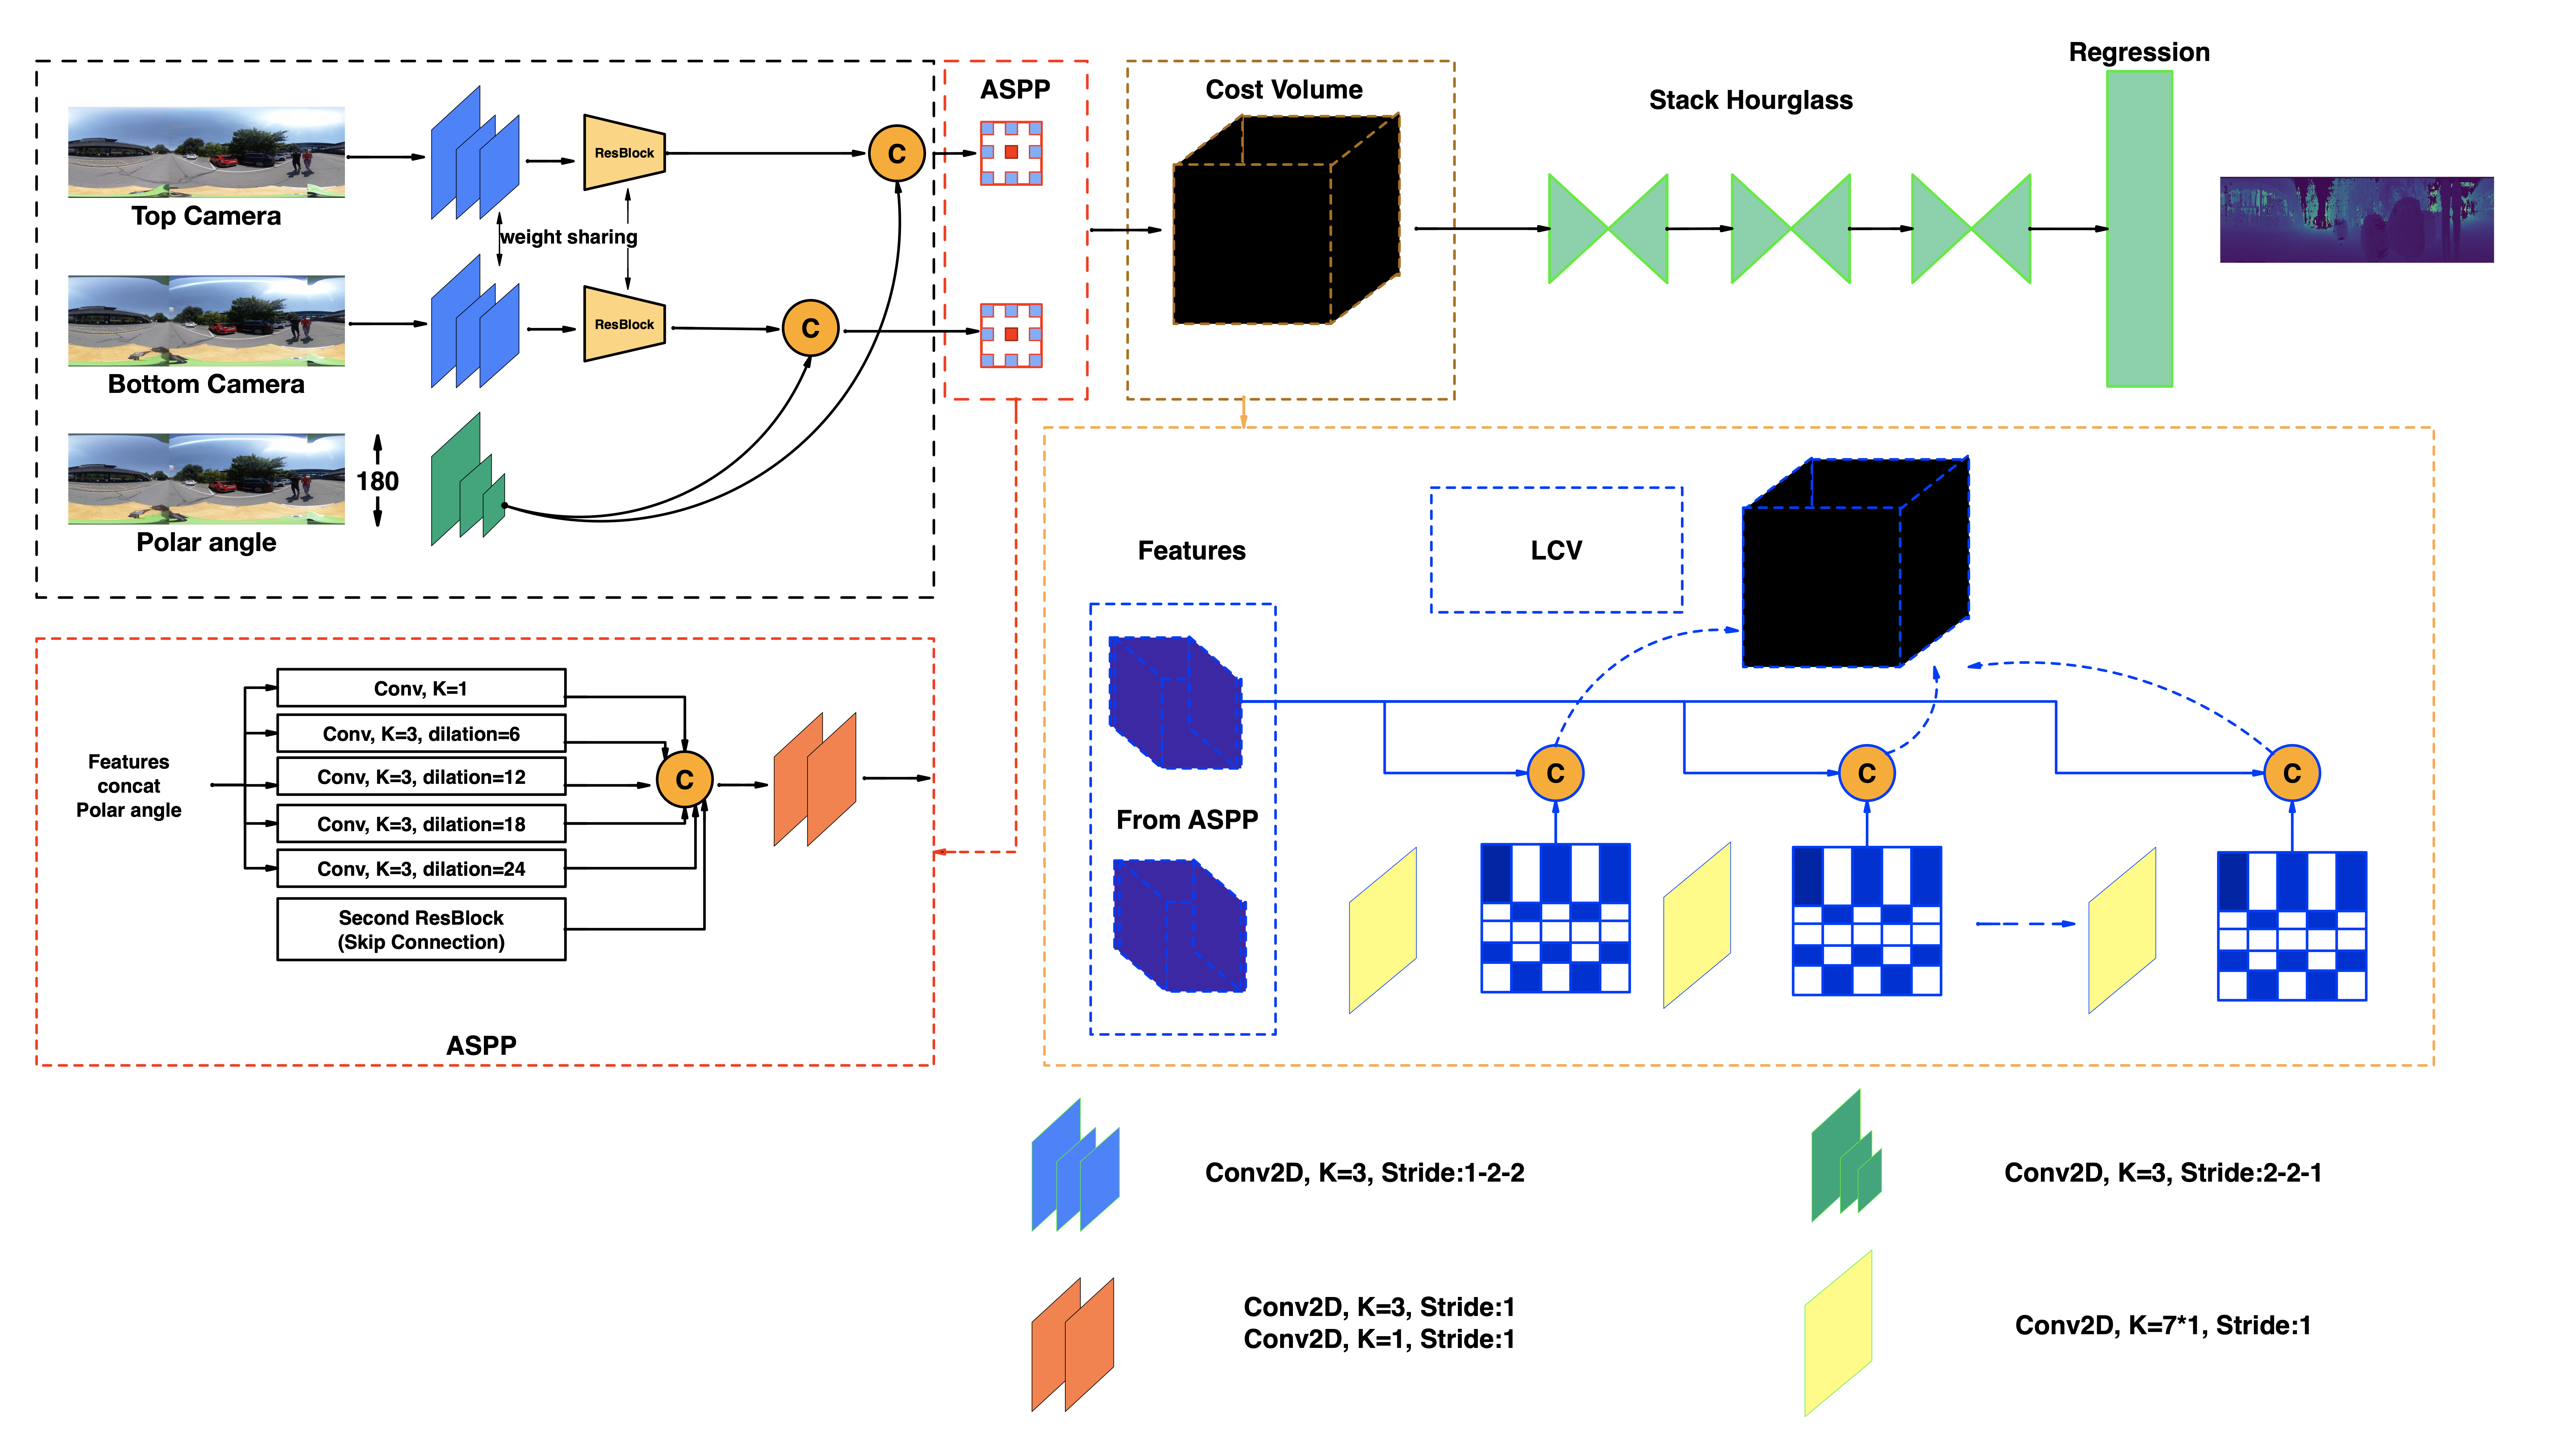
\includegraphics[scale=0.17, angle=90]{Images/arch2.png}
\caption{The network primarily comprises three components: a) a dual-branch feature extractor that combines stereo equirectangular images with polar angles in a late fusion setting, b) an ASPP module designed to expand the receptive field, and c) a learnable cost volume that accommodates the nonlinear spherical projection. A Stacked-Hourglass module is employed to generate the final disparity map.}
\label{fig:felix2}
\end{figure}
\end{landscape}


\vspace{1cm}
\begin{table}
\centering
\caption{Parameters of the Feature extractor architecture.}\label{table:fea}
\begin{tabular}{ |p{3cm}|p{3cm}|p{3cm}| }
\hline
\multicolumn{3}{|c|}{Feature extractor} \\
\hline
Name&  Layer setting& Output dimension\\
\hline
Input &  & $H\times W \times 3$ \\
\hline
\multicolumn{3}{|c|}{CNN} \\
\hline
First\_Conv0 & $3 \times 3, 32$   & $\frac{H}{2} \times \frac{W}{2} \times 32$ \\
\hline
First\_Conv1 & $3 \times 3, 32$   & $\frac{H}{2} \times \frac{W}{2} \times 32$ \\
\hline
First\_Conv2 & $3 \times 3, 32$   & $\frac{H}{2} \times \frac{W}{2} \times 32$ \\
\hline
First\_Conv3 & $3 \times 3, 32$   & $\frac{H}{2} \times \frac{W}{2} \times 32$ \\
\hline
Layer\_1 &  $\begin{bmatrix}
            3 \times 3, 32 \\
            3 \times 3, 32 
            \end{bmatrix} \times 3$
    & $\frac{H}{2} \times \frac{W}{2} \times 32$ \\
\hline
Layer\_2 &  $\begin{bmatrix}
            3 \times 3, 64 \\
            3 \times 3, 64 
            \end{bmatrix} \times 16$
    & $\frac{H}{4} \times \frac{W}{4} \times 64$ \\
\hline
Layer\_3 &  $\begin{bmatrix}
            3 \times 3, 128 \\
            3 \times 3, 128 
            \end{bmatrix} \times 3$
    & $\frac{H}{4} \times \frac{W}{4} \times 128$ \\
\hline
Layer\_4 &  $\begin{bmatrix}
            3 \times 3, 64 \\
            3 \times 3, 64 
            \end{bmatrix} \times 3$
    & $\frac{H}{4} \times \frac{W}{4} \times 128$  \\
\hline
\multicolumn{3}{|c|}{Polar branch} \\
\hline
Polar & $\begin{bmatrix}
            3 \times 3, 64 \\
            3 \times 3, 64 
            \end{bmatrix} \times 3$ & $\frac{h}{4} \times \frac{w}{4} \times 32$  \\
\hline
 
Concat &  & $\frac{H}{4} \times \frac{W}{4} \times 160$  \\
\hline
\multicolumn{3}{|c|}{ASPP} \\
\hline
ASPP\_1 & $1 \times 1, 32$ & $\frac{H}{4} \times \frac{W}{4} \times 32$  \\
\hline
ASPP\_2 & $1 \times 1, 32$ & $\frac{H}{4} \times \frac{W}{4} \times 32$  \\
\hline
ASPP\_3 & $1 \times 1, 32$ & $\frac{H}{4} \times \frac{W}{4} \times 32$  \\
\hline
ASPP\_4 & $1 \times 1, 32$ & $\frac{H}{4} \times \frac{W}{4} \times 32$  \\
\hline
ASPP\_5 & $1 \times 1, 32$ & $\frac{H}{4} \times \frac{W}{4} \times 32$  \\
\hline
Concat &  & $\frac{H}{4} \times \frac{W}{4} \times 224$  \\
\hline
Last\_Conv &  $\begin{bmatrix}
            3 \times 3, 128 \\
            3 \times 3, 128 
            \end{bmatrix} \times 2$ & $\frac{H}{4} \times \frac{W}{4} \times 128$  \\
\hline
\end{tabular}
\end{table}





\section{Adding Polar Angle Information}

In equirectangular images, distortion is often overlooked in stereo depth estimation. To tackle this issue, we incorporate the polar angle, which is closely associated with distortion, as additional geometry information in the model input. In order to distinguish geometry data from RGB appearance information, we employ residual blocks for processing the RGB input and utilize three 2D convolutional layers for the polar angle. This approach avoids the direct concatenation of model inputs, as seen in early fusion designs. Subsequently, after feature extraction, the outputs are combined in a process it's called late fusion design. Paper\cite{c20} shows comparative analysis of both early and late fusion designs in the experimental section of the paper and it concludes that late fusion would result in less RMSE. This approach ensures a more comprehensive understanding of the geometric and appearance information in the images, leading to improved stereo depth estimation in equirectangular images.

\section{ASPP}

Atrous Spatial Pyramid Pooling (ASPP)\cite{aspp} is a computer vision technique used to improve the accuracy of semantic image segmentation tasks. The ASPP module applies atrous convolutions at different rates to a feature map and aggregates the resulting feature maps using pyramid pooling. Atrous convolution is a convolution operation where the filter kernel is applied to the input image with gaps between the kernel values. The gaps between the kernel values control the output feature map's spatial resolution, enabling the convolution operation to have a larger receptive field without increasing the number of parameters. Pyramid pooling is a technique where the input feature map is divided into different regions of various sizes, and the features within each region are pooled to generate a fixed-length vector for each region. The fixed-length vectors from each region are concatenated to form the final feature vector, allowing the network to capture features at multiple scales and improving the accuracy of the segmentation.

The ASPP module uses different dilation rates to capture features at different scales. By applying atrous convolution at different rates, the ASPP module can aggregate information from a broader range of spatial scales, enabling the network to capture both fine-grained and coarse features. The ASPP module's output is then concatenated with the original feature map to produce the final feature map, which is used for semantic segmentation. The ASPP module has been successfully applied in various computer vision tasks, including stereo depth estimation, as demonstrated by Jiang et al. they described how they used the ASPP module to capture features at different scales and concatenate them with the original feature map to produce the final feature map, resulting in improved accuracy of their stereo depth estimation task.


Considering one-dimensional signals first, the output \textit{y[i]} of atrous convolution of a 1-D input signal \textit{x[i]} with a filter \textit{w[k]} of length \textit{K} is defined as:

\begin{equation}\label{eq:41}
\begin{flalign*}
         y[i] = \sum_{k=1}^{K} x[i+r.k]w[k].
    \end{flalign*}
\end{equation}

The rate parameter r corresponds to the stride with which the input signal would be sampled. Standard convolution is a special case for rate r = 1. figure \ref{fig:ASPP1} illustrate it. 

\begin{figure*}[h] %this figure will be at the right
    \centering
    % width=\linewidth
    \includegraphics[scale=0.3]{Images/ASPP1.png}
    \caption{Illustration of atrous convolution in 1-D. (a) Sparse feature extraction with standard convolution on a low resolution input feature map. (b) Dense feature extraction with atrous convolution with rate r = 2, applied on a high resolution input feature map.}
    \label{fig:ASPP1}
\end{figure*}



Atrous convolution also allows us to arbitrarily enlarge the field-of-view of filters at any DCNN layer. The DeepLab-ASPP approach is inspired by the R-CNN spatial pyramid pooling method and uses multiple parallel atrous convolutional layers with different sampling rates. Features are extracted for each sampling rate, processed in separate branches, and fused to generate the final result. This approach generalizes the DeepLab-LargeFOV variant and has been shown to accurately and efficiently classify regions of arbitrary scales. Multiscale Image Representations using Atrous Spatial Pyramid Pooling is illustrated in figure\ref{fig:ASPP2}.

\begin{figure*}[h] %this figure will be at the right
    \centering
    % width=\linewidth
    \includegraphics[width=\linewidth]{Images/ASPP3.png}
    \caption{Atrous Spatial Pyramid Pooling (ASPP). To classify the center pixel (orange), ASPP exploits multi-scale features by employing multiple parallel filters with different rates. The effective Field-Of-Views are shown in different colors.}
    \label{fig:ASPP2}
\end{figure*}

\section{Cost Volume}
Cost Volume is a fundamental concept in computer vision, particularly for stereo matching and depth estimation tasks. It is a 3D data structure representing the matching costs (or similarity) between corresponding pixels or regions in a pair of images, typically stereo images, at different disparity levels. To compute the Cost Volume, a similarity metric such as the Sum of Absolute Differences (SAD), Sum of Squared Differences (SSD), Normalized Cross-Correlation (NCC), or the Census Transform is selected. Matching costs are calculated for each pixel in the reference image and its corresponding pixels in the target image at different disparity levels, and these costs are stored in the Cost Volume.

In some implementations, a 4D cost volume concatenates left feature maps with their corresponding right feature maps across each disparity level. This results in a structure with dimensions (height × width × disparity × feature size). This approach uses Spatial Pyramid Pooling (SPP) features to enhance stereo-matching.

A critical step in stereo matching is constructing a 3D cost volume by computing matching costs at pre-defined disparity levels with a fixed step size. In typical 3D cost volumes, the step size is one pixel. However, with the distortion introduced by equirectangular projection, the per-pixel step size is inconsistent with the geometry information from the polar angle input. To address this issue, a novel learnable cost volume (LCV) can be introduced using a shifting filter, which searches for the optimal step size in "degree unit" to construct the optimal cost volume.

The LCV \cite{c20}is designed with a shifting filter via a 7x1 Conv2D layer, allowing for vertical shifting and retaining the full view of equirectangular images. The best-shifting step size of the feature map is learned through convolution. Replicated padding is applied instead of zero padding before each convolution to retain boundary information.

The minimum matching cost across all disparity levels in the Cost Volume is identified to estimate the disparity for each pixel in the reference image. The disparity level corresponding to the minimum cost is considered the best match, and the depth can be inferred from the disparity through triangulation. By analyzing and processing the Cost Volume, depth estimation, and stereo matching algorithms can estimate the depth or disparity maps for various computer vision tasks, such as 3D reconstruction, object detection, and scene understanding.

\section{3D CNN}
A regularization method is proposed to refine disparity estimates from a disparity cost volume that considers contextual information. Due to the imperfections in matching costs between unaries, even with deep feature representations, the aim is to regularize and improve the cost volume, particularly in regions with uniform pixel intensity.

Three-dimensional (3D) convolutional operations filter and refine the cost volume representation. 3D convolutions can learn feature representations across height, width, and disparity dimensions. To address the computational burden of 3D convolutions, a deep encoder-decoder architecture with sub-sampling and residual layers is used to leverage context and reduce computational requirements.

The proposed 3D CNN architecture for cost volume regularization involves a stacked hourglass \cite{stack} (encoder-decoder) architecture consisting of repeated top-down/bottom-up processing and intermediate supervision. The hourglass design is motivated by capturing information at every scale. While local evidence is essential for identifying features like faces and hands, a final pose estimate requires a coherent understanding of the full body. The person’s orientation, the arrangement of their limbs, and the relationships of adjacent joints are among the many cues that are best recognized at different scales in the image. The hourglass is a simple, minimal design that can capture and combine all these features to output pixel-wise predictions. 
The architecture is designed to capture information at every scale, essential for tasks like human pose estimation, where both local and global context is important. The Hourglass architecture uses a single pipeline with skip layers to preserve spatial information at each resolution. It processes features down to very low resolutions and then branches off to apply more convolutions at the original pre-pooled resolution. The architecture contains twelve 3x3x3 convolutional layers and uses Spatial Pyramid Pooling (SPP) to involve different levels of features. The stacked hourglass architecture has three main networks, each generating a depth map, with the total loss being the weighted summation of the three losses during training, architecture of stack-hour-glass is shown in Figure\ref{}.

\begin{figure*}[h] 
    \centering
    % width=\linewidth
    \includegraphics[width=\linewidth]{Images/stack.png}
    \caption{Complete Stack hour-glass architecture\cite{c16}.}
    \label{fig:ASPP2}
\end{figure*}

For up-sampling, a 3D transposed convolution is employed, and bilinear interpolation is used to restore the cost volume back to its original size. Higher-resolution feature maps are added before up-sampling to retain high-frequency information and spatial accuracy. The final disparity map is the last of the three outputs during the testing phase.

The stacked hourglass is adopted as the 3D Encoder-Decoder, and regression is used to calculate continuous depth values. This approach is reported to be more robust than classification-based stereo-depth estimation methods. The smooth L1 loss with the ground truth depth is employed for the loss function.

The proposed approach combines 3D convolutions, deep encoder-decoder architecture, stacked hourglass architecture, and SPP to refine and regularize the depth cost volume, effectively considering context information and improving stereo performance\cite{c15,c16}.


\section{Depth Regression}


A final cost volume is produced from the matching cost unaries in typical stereo algorithms. Depth estimation can be done by performing an argmin operation over the cost volume's depth dimension. However, this operation has two significant drawbacks: 
\begin{itemize}
    \item it is discrete and is unable to produce sub-pixel disparity estimates
    \item  it is not differentiable and therefore unable to be
trained using back-propagation.
\end{itemize}

A soft argmin operation is defined to address these limitations, which is both fully differentiable and capable of regressing a smooth depth estimate. First, the predicted costs (\textit{c\textsub{d}} for each depth, \textit{d}) from the cost volume are converted to a probability volume by taking the negative of each value. The probability volume is then normalized across the depth dimension with the softmax operation, $\sigma$(.). The sum of each depth, \textit{d}, weighted by its normalized probability, is taken. This operation is fully differentiable and allows for training and regressing depth estimates.
\[\hat{d} = \sum\limits_{d=0}^{D_{max}} d \times \sigma(-c_d) \eqno{(4.1)}\]
It is important to note that a similar function was first introduced in another work and referred to as a soft-attention mechanism. In this case, it is applied to the stereo regression problem. However, compared to the argmin operation, the soft argmin output is influenced by all values, making it susceptible to multi-modal distributions. Consequently, the output may not take the most likely value but will estimate a weighted average of all modes. To overcome this limitation, the network's regularization is relied upon to produce a disparity probability distribution that is predominantly unimodal. The network can also pre-scale the matching costs to control the normalized post-softmax probabilities' peakiness (sometimes called temperature). Batch normalization is explicitly omitted from the final convolution layer in the unary tower to allow the network to learn this from the data \cite{t1, c20,c16}.

\section{Loss}

Because of the depth regression, we adopt the smooth L1 loss function to train the proposed PSMNet. Smooth L1 loss is widely used in bounding box regression for object detection because of its robustness and low sensitivity to outliers, as compared to L2 loss. When the regression targets are unbounded, training with L2 loss can require careful tuning of learning rates in order to prevent exploding
gradient. The loss function is defined as

\begin{equation}\label{eq:loss}
\begin{flalign*}
         L(d,\hat{d}) = \frac{1}{N} \sum_{i=1}^{N} smooth\textsub{L\textsub{1}}(d - \hat{d}\textsub{i})
    \end{flalign*}
\end{equation}

in which:


\begin{equation}\label{eq:loss2}
    % \begin{flalign*}
        \Biggl\{
        \begin{align*}
        0.5x^2&&        &  if |x|<1  \\
        |x| - 0.5 &&      &  O.W   \\    
        \end{align*}
    % \begin{flalign*}
\end{equation}
where N is the number of labeled pixels, \textit{d} is the ground-truth depth, and $\hat{d}$ is the predicted depth\cite{c16}.
% ################################# End Chapter 4 ###################################
%####################################################################################



% ################################# Chapter 5 #######################################
%####################################################################################


\chapter{Experiments and Results }

\section{Dataset and System Configuration}


Due to the complexity and the extensive effort required to stitch, calibrate, and collect real-world RGB images and depth maps, which is not suitable for the training of deep models, and the lack of 360 datasets with real images, [] profited from available 360 datasets, such as Matterport3D  and Stanford3D point clouds. However, as described in Chapter 2, we have gathered our 360 datasets, including real and not rectified images.

The setting of our dataset is a pair of $360^\circ$ top-bottom aligned stereo images with equirectangular projection. In contrast to the commonly used in $360^\circ$ works \cite{ex1,ex2,ex3} the resolution of our images is 1920 in height and 3840 in width. The baseline of our stereo system is set to 20[cm], and the number of data we have collected in datasets for training and validation are 690 and 77, respectively. The reason that we used 10 percent of our Outdoor1 dataset is based on the fact that our dataset includes frames of a video with 10[f/s], so we decided to use one frame per every ten frames that have been taken in order to have more consistent training and to prevent similarities and repetitiveness. Each data consists of three components, an RGB-image pair, and depth. 

Our setup is vertically aligned with full-resolution images of 3840$\times$1920. These images include the sky and part of the setup (top of the box) can be seen mainly in the images from the bottom camera. These textureless regions can cause errors in the training, so we decided to remove them which led to a resolution of 1024$\times$512. 
In addition, the structure of our pair images from the cameras differs from the one exported from Lidar. In order to fix this issue, algorithm 1 was applied. 


\begin{algorithm}
\caption{transformer}
\begin{algorithmic}[1]
\Function{transf}{$A \in \mathbb{R}^{m \times n \times p}, k \in \mathbb{N}$}
    \State Initialize $B \in \mathbb{R}^{m \times n \times p}$ with zeros
    \For{$i \gets 0$ to $m - 1$}
        \For{$j \gets 0$ to $n - 1$}
            \For{$c \gets 0$ to $p - 1$}
                \State $B(i, j, c) \gets A(i, (j - k) \mod n, c)$
            \EndFor
        \EndFor
    \EndFor
    \State \Return{$B$}
\EndFunction
\end{algorithmic}
\end{algorithm}

\begin{figure*}[h!] %this figure will be at the right
    \centering
    \includegraphics[width=\linewidth]{Images/diag.png}
    \caption{Code diagram.}
    \label{fig:diag}
\end{figure*}


We extracted our ground-truth images with 16 bits which caused each pixel to have a value between 0 to $2^{(15)}$. In order to normalize values, we tried different approaches. However, based on the manual of Ouster, the value of each pixel would present the distance in millimeters, so we decided to convert these values to meters to reduce the range. 

Furthermore, For a convolutional layer to work with cylindrical input, it must preserve this horizontal wrapping property, rather than using zero-padding as is typical. Horizontal wrapping can be done by padding the right side of the tensor with columns from the left and vice-versa. 

\section{Metrics}
\textbf{MAE} stands for \textit{Mean Absolute Error}, \textbf{MSE} stands for \textit{Mean Squared Error}, and \textbf{RMSE} stands for \textit{Root Mean Squared Error}. These are common evaluation metrics used to assess the performance of regression models, specifically in terms of how well they can predict continuous values.

\textit{Mean Absolute Error (MAE)} is an easy-to-understand metric that calculates the average absolute difference between the predicted and true values. The formula for calculating MAE is:

\begin{equation}
\text{MAE} = \frac{1}{n} \sum_{i=1}^n |y_i - \hat{y}_i|
\end{equation}

where $n$ is the number of data points, $y_i$ represents the true value, and $\hat{y}_i$ represents the predicted value. The metric takes the absolute value of the difference to ensure all errors are positive, and then computes the average of these values.

\textit{Mean Squared Error (MSE)} is another popular metric that calculates the average of the squared differences between the predicted and true values. The formula for calculating MSE is:

\begin{equation}
\text{MSE} = \frac{1}{n} \sum_{i=1}^n (y_i - \hat{y}_i)^2
\end{equation}

By squaring the differences, MSE emphasizes larger errors, which can be useful in situations where large deviations are particularly undesirable.

\textit{Root Mean Squared Error (RMSE)} is simply the square root of the MSE. The formula for calculating RMSE is:

\begin{equation}
\text{RMSE} = \sqrt{\text{MSE}}
\end{equation}

RMSE shares the same unit as the predicted and true values, making it easier to interpret than MSE. It also emphasizes larger errors like MSE, but by taking the square root, it balances between the sensitivity of MSE and the interpretability of MAE. When choosing the appropriate metric for your thesis, consider the specific context and goals of your project, as well as the benefits and limitations of each metric.

\section{Experimental Setting}
In the course of this project, we utilized an NVIDIA GTX 580 GPU to train our deep learning models for stereo depth estimation. The choice of this powerful GPU enabled us to efficiently perform the necessary computations and accelerate the training process. Over a total of 500 epochs, we were able to fine-tune the model parameters and achieve convergence, ensuring optimal performance on our novel dataset of real-world stereo 360-degree images. 




\begin{table}[h]
\centering
\caption{Comparison of 360SD-Net architecture and ours on the dataset Outdoor\_1.  }
\label{table:sample}
\begin{tabular}{|l | c | r} % Alignment: left, center, right
\toprule
\textbf{architecture}  & \textbf{RMSE} \\
\midrule
360SD-Net &  $2.3 \times 10^3$ \\
Ours & 0.9 \\
\bottomrule
\end{tabular}
\end{table}






\begin{table}[ht]
\centering
\caption{Ablation study of out architecture}
\label{table:sample}
\begin{adjustbox}{width=1\textwidth}
\begin{tabular}{| c | c | c | c | c | c |} % Alignment: left, center, right, center
\hline
\multicolumn{3}{| c | }{\textbf{Network setting}} &\textbf{Dataset} & \textbf{Val Err}  & \textbf{ RMSE} } \\
\hline

\hline
Input size & polar angle & Max Depth &  &  &  \\
\hline
 256\times256 & \checkmark & 80 & Outdoor1,2  & 1.14 & 3.2 \\ % 2004
\hline
256\times256 & \times & 80 &  Outdoor1,2  & 1.2 & 3.22\\ % 2005
\hline
256\times512 & \checkmark & 80 &Outdoor1,2  & 1.13 & 3.18\\ % 2007
\hline
\hline
\end{tabular}
\end{adjustbox}
\end{table}



\begin{table}[h]
\centering
\caption{Ablation study of Max depth parameter. }
\label{table:sample}
\begin{tabular}{|l | c | r |} % Alignment: left, center, right
\toprule
\textbf{Max Depth }  & \textbf{Val loss} & \textbf{RMSE} \\
\midrule
80 & 3.009 & 0.99  \\
150 & 3.015 & 1.014\\
\bottomrule
\end{tabular}
\end{table}

\section{Performance}

Our primary objective was to investigate the potential improvements that could be achieved by introducing new data and training our model accordingly. The results have demonstrated a marked enhancement in the overall performance, surpassing the capabilities of the 360SD-Net model when applied to our dataset.

Upon introducing the new data, we meticulously trained our model, ensuring that it was able to effectively learn and adapt to the unique characteristics presented. This process was crucial in maximizing the model's potential and optimizing its predictive capabilities. The subsequent analysis revealed that our model exhibited a superior performance, consistently outperforming the 360SD-Net model across various metrics. 

\section{Ablation study}
Our findings indicate that using larger input images significantly improves the performance of the depth estimation models. This can be attributed to the fact that larger images retain more detailed information and provide a higher resolution for the model to work with. This allows the model to capture more subtle variations in depth and enables it to produce more accurate depth estimates. As a result, we suggest that using higher resolution input images can be beneficial for our depth estimation tasks, provided that the computational resources are available to handle the increased complexity.

On the other hand, our ablation study revealed that the contribution of polar angle information to the overall performance of our model appears to be minimal. In fact, the results suggest that incorporating polar angle information may not be necessary in our specific case. This finding implies that our model is able to learn relevant features and accurately estimate depth without relying on polar angle information. This insight can potentially simplify the model architecture and reduce the computational burden, allowing for faster training and inference times.



\begin{figure*}[h!] %this figure will be at the right
    \centering
    \includegraphics[width=\linewidth]{Images/re(1).png}
    \caption{Qualitative result of our different experiments.}
    \label{fig:l}
\end{figure*}

\begin{figure*}[h!] %this figure will be at the right
    \centering
    \includegraphics[width=\linewidth]{Images/ress.png}
    \caption{Qualitative result of our different experiments.}
    \label{fig:l}
\end{figure*}

\begin{figure*}[h!] %this figure will be at the right
    \centering
    \includegraphics[width=\linewidth]{Images/g_1.png}
    \caption{a) Validation loss, b)Log of RMSE}
    \label{fig:loss}
\end{figure*}


Figure\ref{fig:loss} shows the validation loss of the trained model. The model has not reached an overfit which implies one of these two reasons, either the model is too deep for this dataset or the number of data is limited. Based on our work, it can be said that the number of data is limited and has to be expanded in number and scene in order to generalize the architecture. 
% ################################# End Chapter 5 ###################################
%####################################################################################
\chapter{Conclusions}
% In conclusion, one of the key observations from our research is the importance of diversity in the dataset used for training and evaluating depth estimation models. Our current dataset, while presenting a new challenge for depth estimation in stereo 360$^\circ$ images, is not diverse enough in terms of the number of samples and the variety of scenes represented. This limitation may affect the generalizability of our findings and the performance of the models when applied to different real-world scenarios.

% To address this issue, future work could focus on expanding the dataset by increasing the number of samples and capturing images from a wider range of scenes, environments, and conditions. By doing so, the models can be trained on a more representative dataset, which would potentially improve their ability to generalize to various real-world situations. This, in turn, would lead to better performance and more accurate depth estimation in diverse applications, ultimately contributing to the advancement of stereo depth estimation from stereo 360$^\circ$ images.

% Another peculiarity of the dataset is the resolution of Lidars which comes from the Ouster OS-1. The maximum resolution of this Lidar is 1024 64; compared to other datasets, our dataset has a very low resolution in height. This low resolution in ground truth caused us to lose information about textureless regions, such as the sky. Utilizing the OS-2 model can enhance the exported dataset in that term and may impact the final result. 
In conclusion, our research highlights the critical role of diversity in the dataset used for training and evaluating depth estimation models. Although our current dataset presents a novel challenge for depth estimation in stereo 360$^\circ$ images, it falls short in terms of the number of samples and the variety of scenes represented. This limitation could potentially affect the generalizability of our findings and the performance of the models in diverse real-world scenarios.

To overcome this issue, future work should concentrate on augmenting the dataset by increasing the number of samples and capturing images from a broader range of scenes, environments, and conditions. By training the models on a more representative dataset, their generalization capabilities can be improved, leading to better performance and more accurate depth estimation across various applications. This would ultimately contribute to the advancement of stereo depth estimation in the context of stereo 360$^\circ$ images.

Another aspect worth considering is the resolution of the Lidars used in our dataset, which are sourced from the Ouster OS-1. With a maximum resolution of 1024x64, our dataset exhibits a relatively low height resolution compared to other datasets. This low resolution in ground truth data results in the loss of information about textureless regions, such as the sky. Upgrading to the OS-2 model could enhance the quality of the dataset and potentially impact the final depth estimation results. By addressing these limitations, we hope to further refine the performance of depth estimation models and broaden their applicability in real-world situations.
\backmatter
\phantomsection

% \section*{Bibliography}
% \bibliography{references}

\begin{thebibliography}{99}

% SF3D
\bibitem{ref:SF3D} Curless, B., Levoy, M. (1996). A volumetric method for building complex models from range images. In Proceedings of the 23rd Annual Conference on Computer Graphics and Interactive Techniques (pp. 303-312).

\bibitem{ref:rectification3} Fusiello, Andrea, Emanuele Trucco, and Alessandro Verri. "A compact algorithm for rectification of stereo pairs." Machine vision and applications 12 (2000): 16-22.

\bibitem{c1}Scharstein, D. and Szeliski, R., 2002. A taxonomy and evaluation of dense two-frame stereo correspondence algorithms. International journal of computer vision, 47(1), pp.7-42.

\bibitem{ref:Spherical stereo}
Li, Shigang, and Kiyotaka Fukumori. “\textit{Spherical stereo for the construction of immersive VR environment}“, IEEE Proceedings. VR 2005. Virtual Reality, 2005.. IEEE, 2005.

\bibitem{ref:Binocular spherical}
Li, Shigang. “\textit{Binocular spherical stereo}“, IEEE Transactions on intelligent transportation systems 9.4 (2008): 589-600.




% \bibitem{c17}Li, S., 2008. Binocular spherical stereo. IEEE Transactions on intelligent transportation systems, 9(4), pp.589-600.
\bibitem{ref:d1} Geiger, A., Lenz, P., Stiller, C., Urtasun, R. (2012). Vision meets robotics: The KITTI dataset. The International Journal of Robotics Research, 32(11), 1231-1237.


% chapter 3
\bibitem{c18} Kim, H. and Hilton, A., 2013. 3d scene reconstruction from multiple spherical stereo pairs. International journal of computer vision, 104(1), pp.94-116.

\bibitem{c13}Zagoruyko, S. and Komodakis, N., 2015. Learning to compare image patches via convolutional neural networks. In Proceedings of the IEEE conference on computer vision and pattern recognition (pp. 4353-4361).

\bibitem{c25}Frogner, C., Zhang, C., Mobahi, H., Araya, M. and Poggio, T.A., 2015. Learning with a Wasserstein loss. Advances in neural information processing systems, 28.

\bibitem{t1}R. Girshick. Fast R-CNN. In Proceedings of the IEEE inter- national conference on computer vision, pages 1440–1448, 2015.

\bibitem{c12}J.ZbontarandY.LeCun,“Stereo matching by training a convolutional neural network to compare image patches,” Journal of Machine Learning Research, vol. 17, pp. 1–32, 2016. 



\bibitem{c19}Pathak, S., Moro, A., Yamashita, A. and Asama, H., 2016, October. Dense 3D reconstruction from two spherical images via optical flow-based equirectangular epipolar rectification. In 2016 IEEE International Conference on Imaging Systems and Techniques (IST) (pp. 140-145). IEEE.

\bibitem{c19}Pathak, S., Moro, A., Yamashita, A. and Asama, H., 2016, October. Dense 3D reconstruction from two spherical images via optical flow-based equirectangular epipolar rectification. In 2016 IEEE International Conference on Imaging Systems and Techniques (IST) (pp. 140-145). IEEE.

\bibitem{ref:d2} Mayer, N., Ilg, E., Häusser, P., Fischer, P., Cremers, D., Dosovitskiy, A., Brox, T. (2016). A large dataset to train convolutional networks for disparity, optical flow, and scene flow estimation. In Proceedings of the IEEE Conference on Computer Vision and Pattern Recognition (pp. 4040-4048).

\bibitem{c21}Ohashi, A., Yamano, F., Masuyama, G., Umeda, K., Fukuda, D., Irie, K., Kaneko, S., Murayama, J. and Uchida, Y., 2017, December. Stereo rectification for equirectangular images. In 2017 IEEE/SICE International Symposium on System Integration (SII) (pp. 535-540). IEEE.

% psm2
\bibitem{c15}Alex Kendall, Hayk Martirosyan, Saumitro Dasgupta, Peter Henry, Ryan Kennedy, Abraham Bachrach, and Adam Bry. End-to-end learning of geometry and context for deep stereo regression. In ICCV, 2017, pages 66–75, 2017. 1, 2, 3, 7 

\bibitem{aspp} Chen, Liang-Chieh, et al. "Deeplab: Semantic image segmentation with deep convolutional nets, atrous convolution, and fully connected crfs." IEEE transactions on pattern analysis and machine intelligence 40.4 (2017): 834-848.

\bibitem{ref:rectification2} Ohashi, Akira, et al. "Stereo rectification for equirectangular images." 2017 IEEE/SICE International Symposium on System Integration (SII). IEEE, 2017.

\bibitem{ref:rectification1} Aghayari, S., et al. “\textit{Geometric calibration of full spherical panoramic Ricoh-Theta camera}“. ISPRS Annals of the Photogrammetry, Remote Sensing and Spatial Information Sciences IV-1/W1 (2017) 4 (2017): 237-245.

% MP3D
\bibitem{ref:d3} Chang, A. X., Dai, A., Funkhouser, T., Halber, M., Niessner, M., Savva, M., ... Song, S. (2017). Matterport3D: Learning from RGB-D data in indoor environments. In Proceedings of the International Conference on 3D Vision (3DV) (pp. 667-676).

\bibitem{c21}Ohashi, A., Yamano, F., Masuyama, G., Umeda, K., Fukuda, D., Irie, K., Kaneko, S., Murayama, J. and Uchida, Y., 2017, December. Stereo rectification for equirectangular images. In 2017 IEEE/SICE International Symposium on System Integration (SII) (pp. 535-540). IEEE.

\bibitem{c22}Aghayari, S., Saadatseresht, M., Omidalizarandi, M. and Neumann, I., 2017. Geometric calibration of full spherical panoramic Ricoh-Theta camera. ISPRS Annals of the Photogrammetry, Remote Sensing and Spatial Information Sciences IV-1/W1 (2017), 4, pp.237-245.

\bibitem{c23}Chang, A., Dai, A., Funkhouser, T., Halber, M., Niessner, M., Savva, M., Song, S., Zeng, A. and Zhang, Y., 2017. Matterport3d: Learning from rgb-d data in indoor environments. arXiv preprint arXiv:1709.06158.

% psmnet
\bibitem{c16}Chang, J.R. and Chen, Y.S., 2018. Pyramid stereo matching network. In Proceedings of the IEEE conference on computer vision and pattern recognition (pp. 5410-5418).

\bibitem{c20}Wang, N.H., Solarte, B., Tsai, Y.H., Chiu, W.C. and Sun, M., 2020, May. 360sd-net: 360 stereo depth estimation with learnable cost volume. In 2020 IEEE International Conference on Robotics and Automation (ICRA) (pp. 582-588). IEEE.

% 360sdnet
\bibitem{c20}Wang, N.H., Solarte, B., Tsai, Y.H., Chiu, W.C. and Sun, M., 2020, May. 360sd-net: 360 stereo depth estimation with learnable cost volume. In 2020 IEEE International Conference on Robotics and Automation (ICRA) (pp. 582-588). IEEE.

\bibitem{ref:ouster}
Ouster. \textit{Ouster Studio User Guide}. Ouster, 2021. \url{https://data.ouster.io/downloads/software-user-manual/software-user-manual-v2p0.pdf}

\bibitem{ref:s3}
Zheng, Yuanzhou, et al. “\textit{Recognition and depth estimation of ships based on binocular stereo vision}“. Journal of Marine Science and Engineering 10.8 (2022): 1153.






% ---------INtro-------------------------------------------
\bibitem{int1} Jeffrey Hawke, E Haibo, Vijay Badrinarayanan, Alex Kendall, et al. “Reimagining an autonomous vehicle”. In: arXiv preprint arXiv:2108.05805 (2021).

\bibitem{int2} World Health Organization. Infographics on Road Traffic Injuries. Ed. by World Health Organization. 2021. url{https://www.who.int/news-room/fact-sheets/detail/road-traffic- injuries}.

\bibitem{int3} U.S. Department of Transportation. Automated Driving Systems 2.0, A Vision for Safety. 2021. url{https://www.nhtsa.gov/sites/nhtsa.gov/files/documents/13069a-ads2.0_ 090617_v9a_tag.pdf}.

\bibitem{int4} Daniel Holland-Letz, Benedikt Kloss, Matthias Kässer, and Thibaut Müller. Start me up: Where mobility investments are going. Tech. rep. McKinsey & Company, 2019.

\bibitem{int5} Mel Siegel. “The sense-think-act paradigm revisited”. In: 1st International Workshop on Robotic Sensing, 2003. ROSE’03. IEEE. 2003, 5–pp.

\bibitem{int6} John Krafcik. Waymo is opening its fully driverless service to the general public in Phoenix. Ed. by Blog Post. 2020. URL: https://blog.waymo.com/2020/10/waymo-is- opening-its-fully-driverless.html.

\bibitem{int7} Wayve Ltd. Unlocking Markets Faster: Building AVs that Generalise. Ed. by Blog Post. 2021. URL: https://wayve.ai/blog/unlocking-markets-faster-building-avs-that-generalise/.

\bibitem{int8} Alex Krizhevsky, Ilya Sutskever, and Geoffrey E Hinton. “Imagenet classification with deep convolutional neural networks”. In: Advances in neural information processing systems (NeurIPS) 25 (2012), pp. 1097–1105.

\bibitem{int9} Alex Krizhevsky, Ilya Sutskever, and Geoffrey E Hinton. “ImageNet Classification with Deep Convolutional Neural Networks”. In: Advances in Neural Information Processing Systems. Ed. by F. Pereira, C. J. C. Burges, L. Bottou, and K. Q. Weinberger. Vol. 25. Curran Associates, Inc., 2012, pp. 1097–1105. url{https://proceedings.neurips.cc/paper/ 2012/file/c399862d3b9d6b76c8436e924a68c45b-Paper.pdf}.

\bibitem{int10} Jamie Shotton, Andrew Blake, and Roberto Cipolla. “Contour-based learning for object detection”. In: Tenth IEEE International Conference on Computer Vision (ICCV’05) Volume 1. Vol. 1. IEEE. 2005, pp. 503–510.

\bibitem{int11} Joseph Redmon, Santosh Divvala, Ross Girshick, and Ali Farhadi. “You only look once: Unified, real-time object detection”. In: the IEEE conference on computer vision and pattern recognition. 2016, pp. 779–788.

\bibitem{int12} Jamie Shotton, Ross Girshick, Andrew Fitzgibbon, Toby Sharp, Mat Cook, Mark Finoc- chio, Richard Moore, Pushmeet Kohli, Antonio Criminisi, Alex Kipman, et al. “Efficient human pose estimation from single depth images”. In: IEEE transactions on pattern analysis and machine intelligence 35.12 (2012), pp. 2821–2840.

\bibitem{int13} Zhe Cao, Gines Hidalgo Martinez, Tomas Simon, Shih-En Wei, and Yaser A Sheikh. “OpenPose: realtime multi-person 2D pose estimation using Part Affinity Fields”. In: IEEE transactions on pattern analysis and machine intelligence (TPAMI) (2019).

\bibitem{int14} Xiaozhi Chen, Kaustav Kundu, Ziyu Zhang, Huimin Ma, Sanja Fidler, and Raquel Urta- sun. “Monocular 3d object detection for autonomous driving”. In: The IEEE Conference on Computer Vision and Pattern Recognition (CVPR). 2016, pp. 2147–2156.

\bibitem{int15} Xiaozhi Chen, Kaustav Kundu, Yukun Zhu, Andrew G Berneshawi, Huimin Ma, Sanja Fidler, and Raquel Urtasun. “3d object proposals for accurate object class detection”. In: Advances in Neural Information Processing Systems. 2015, pp. 424–432.

\bibitem{int16} Julieta Martinez, Rayat Hossain, Javier Romero, and James J Little. “A simple yet effective baseline for 3d human pose estimation”. In: The IEEE International Conference on Computer Vision (ICCV). IEEE. 2017, pp. 2659–2668.

\bibitem{int17} Jia Deng, Wei Dong, Richard Socher, Li-Jia Li, Kai Li, and Li Fei-Fei. “Imagenet: A large-scale hierarchical image database”. In: 2009 IEEE conference on computer vision and pattern recognition. Ieee. 2009, pp. 248–255.

\bibitem{int18} Andreas Geiger, Philip Lenz, Christoph Stiller, and Raquel Urtasun. “Vision meets Robotics: The KITTI Dataset”. In: International Journal of Robotics Research (IJRR) (2013).

\bibitem{int19} Yan Wang, Wei-Lun Chao, Divyansh Garg, Bharath Hariharan, Mark Campbell, and Kilian Q Weinberger. “Pseudo-lidar from visual depth estimation: Bridging the gap in 3d object detection for autonomous driving”. In: The IEEE Conference on Computer Vision and Pattern Recognition. 2019, pp. 8445–8453.

\bibitem{int20} Yurong You, Yan Wang, Wei-Lun Chao, Divyansh Garg, Geoff Pleiss, Bharath Hariharan, Mark Campbell, and Kilian Q Weinberger. “Pseudo-LiDAR++: Accurate Depth for 3D Object Detection in Autonomous Driving”. In: arXiv preprint arXiv:1906.06310 (2019).

\bibitem{int21} Holger Caesar, Varun Bankiti, Alex H Lang, Sourabh Vora, Venice Erin Liong, Qiang Xu, Anush Krishnan, Yu Pan, Giancarlo Baldan, and Oscar Beijbom. “nuscenes: A multimodal dataset for autonomous driving”. In: The IEEE Conference on Computer Vision and Pattern Recognition. 2020, pp. 11621–11631.

\bibitem{int22} Waymo. Waymo Open Dataset: An autonomous driving dataset. 2019.
\bibitem{int23} R. Kesten et al. Lyft Level 5 AV Dataset 2019. url{https://level5.lyft.com/dataset/. 2019}.

\bibitem{residual}He, Kaiming, et al. "Deep residual learning for image recognition." Proceedings of the IEEE conference on computer vision and pattern recognition. 2016.

\bibitem{relu} V. Nair and G. E. Hinton. Rectified linear units improve restricted boltzmann machines. In ICML, 2010.

\bibitem{stack} Newell, Alejandro, Kaiyu Yang, and Jia Deng. "Stacked hourglass networks for human pose estimation." Computer Vision–ECCV 2016: 14th European Conference, Amsterdam, The Netherlands, October 11-14, 2016, Proceedings, Part VIII 14. Springer International Publishing, 2016.

\bibitem{ex1} C. Sun, C.-W. Hsiao, M. Sun, and H.-T. Chen, “Horizonnet: Learning room layout with 1d representation and pano stretch data augmen- tation,” in The IEEE Conference on Computer Vision and Pattern Recognition (CVPR), June 2019.

\bibitem{ex3} F.-E. Wang, H.-N. Hu, H.-T. Cheng, J.-T. Lin, S.-T. Yang, M.-L. Shih, H.-K. Chu, and M. Sun, “Self-supervised learning of depth and camera motion from 360°videos,” in Asian Conference on Computer Vision. Springer, 2018, pp. 53–68.

\bibitem{ex2} C. Sun, C.-W. Hsiao, M. Sun, and H.-T. Chen, “Horizonnet: Learning room layout with 1d representation and pano stretch data augmen- tation,” in The IEEE Conference on Computer Vision and Pattern Recognition (CVPR), June 2019.

\bibitem{f1} S. Peleg and M. Ben-Ezra, "Panoramic Stereo Imaging," in Proceedings of the 2000 IEEE Conference on Computer Vision and Pattern Recognition (CVPR 2000), vol. 1, pp. 378-383, 2000.

\bibitem{f2} J.Gluckman and S. K. Nayar, "Stereo from Spherical Cameras," in Proceedings of the Seventh IEEE International Conference on Computer Vision, vol. 1, pp. 394-401, 1999.

\bibitem{f3} T. Tuytelaars and L. Van Gool, "Wide Baseline Stereo Matching based on Local, Affinely Invariant Regions," in Proceedings of the 11th British Machine Vision Conference (BMVC 2000), vol. 1, pp. 412-422, 2000.
% -----------------------------------------------------------
% rec




% ------------------------------------------------------------
% arch











\end{thebibliography}

\end{document}